\documentclass[sigconf,dvipsnames]{acmart}
\usepackage[english]{babel}
\usepackage[utf8x]{inputenc}
\usepackage[T1]{fontenc}
\usepackage{relsize}
\usepackage{amsmath,amssymb}
\usepackage{xspace}
%% Useful packages
\usepackage{graphicx}
\usepackage{pdflscape,adjustbox}
\usepackage{multirow}

% \usepackage{multirow}
\usepackage{xcolor}

\usepackage{algorithm}
\usepackage[noend]{algpseudocode}
%\algrenewcommand{\algorithmiccomment}[1]{\hfill\texttt{//} #1}

\usepackage{booktabs} % For formal tables
\usepackage{enumitem}
\usepackage{afterpage,tabularx}
%\usepackage[colorlinks=true, allcolors=blue]{hyperref}
 
\newcommand{\true}{\textsc{true}}
\newcommand{\false}{\textsc{false}}
\newcommand{\NULL}{\textsc{null}}
\newcommand{\NA}{---}
\newcommand{\assign}{\ensuremath{:=}}
\newcommand{\procedure}[1]{\textsf{#1}}
\newcommand{\Inf}{\ensuremath{\infty}}
\DeclareMathOperator*{\argmax}{arg\,max}
\DeclareMathOperator*{\argmin}{arg\,min}


\newcommand{\Prob}{\ensuremath{p}}
\newcommand{\minit}{\ensuremath{m_\text{ini}}\xspace}
%\newcommand{\FEmax}{\ensuremath{\textit{FE}_{\max}}}
\newcommand{\FEmax}{\ensuremath{m}}

\newcommand{\supplement}{\href{http://doi.org/10.5281/zenodo.4500974}{doi:~10.5281/zenodo.4500974}}
\newcommand{\ken}{Kendall's-$\tau$}
%% Revision documents
%\usepackage[dvipsnames]{xcolor}
\usepackage[normalem]{ulem}
% FIXME: \sout is not very good. It cannot handle commands within its argument.
\newcommand{\SuggestEdit}[3][red]{\textcolor{#1}{\sout{#2}}\textcolor{#1}{#3}}
\let\svthefootnote\thefootnote
\newcommand\colorfootnote[2][black]{\def\thefootnote{\color{#1}\svthefootnote}%
  \footnote{\color{#1}#2}\def\thefootnote{\color{black}\svthefootnote}}
\newcommand\RevComment[3][red]{\protect\colorfootnote[#1]{{\textbf{[#2: #3]}}}}
% Command for edits, command for commenting and color
\newcommand\newrevisor[3]{%%
  \colorlet{#1}{#3}
  \expandafter\newcommand\csname#1\endcsname[2]{\SuggestEdit[#1]{##1}{##2}}%%
  \expandafter\newcommand\csname#2\endcsname[1]{\RevComment[#1]{#2}{##1}}%%
}
\newrevisor{manuel}{MANUEL}{Purple}
\newrevisor{ekhine}{EKHINE}{red}
%\usepackage{showframe}

\hyphenation{%%% Merriam-Webster
  di-men-sion-al %%
  op-tical net-works semi-conduc-tor %%
  pher-o-mone non-dom-i-nance %%
  non-dom-i-nat-ed chro-mo-some %%
  sto-chas-tic make-span an-a-lys-ing}

% Copyright
%\setcopyright{none}
%\setcopyright{acmcopyright}
%\setcopyright{acmlicensed}
\setcopyright{rightsretained}
%\setcopyright{usgov}
%\setcopyright{usgovmixed}
%\setcopyright{cagov}
%\setcopyright{cagovmixed}


% DOI
\acmDOI{10.1145/nnnnnnn.nnnnnnn}

% ISBN
\acmISBN{978-x-xxxx-xxxx-x/YY/MM}

% Conference
\acmConference[GECCO '21]{the Genetic and Evolutionary Computation Conference 2021}{July 10--14, 2021}{Lille, France}
\acmYear{2021}
\copyrightyear{2021}

%\acmArticle{4}
\acmPrice{15.00}

\begin{document}
\title{Unbalanced Mallows Models for Optimizing Expensive Black-Box Permutation Problems}
% Double-blind
\author{Double-blind}
% \authornote{Dr.~Trovato insisted his name be first.}
% \orcid{1234-5678-9012}
% \affiliation{%
%   \institution{Institute for Clarity in Documentation}
%   \streetaddress{P.O. Box 1212}
%   \city{Dublin} 
%   \state{Ohio} 
%   \postcode{43017-6221}
% }
% \email{trovato@corporation.com}

% \author{Ekhiñe Irurozki\inst{1} \and Manuel López-Ibáñez\inst{2}\orcidID{0000-0001-9974-1295}}
% \institute{
%    Basque Center for Applied Mathematics\\
%    \email{eirurozki@bcamath.org}
%    \and
%    University of Málaga, Málaga, Spain\\
%    \email{manuel.lopez-ibanez@uma.es}
%  }
%    \renewcommand{\shortauthors}{B. Trovato et al.}
\begin{abstract}
%The abstract should briefly summarize the contents of the paper in
%150--250 words.
  Expensive black-box combinatorial optimization problems arise in practice
  when the objective function is evaluated by means of a simulator or a
  real-world experiment. Since each fitness evaluation is expensive in terms of
  time or resources, only a limited number of evaluations is possible,
  typically several orders of magnitude smaller than in non-expensive problems. In
  this scenario, classical optimization methods such as mixed-integer
  programming and local search are not useful.  In the continuous case,
  Bayesian optimization, in particular using Gaussian processes, has proven
  very effective under these conditions. Much less research is available in the
  combinatorial case. In this paper, we propose and analyze UMM, an
  estimation-of-distribution (EDA) algorithm based on a Mallows probabilistic
  model and unbalanced rank aggregation (uBorda). Experimental results on
  black-box versions of LOP and PFSP show that UMM is able to match, and
  sometimes surpass, the solutions obtained by CEGO, a Bayesian optimization
  algorithm for combinatorial
  optimization. %, specially when the budget of solutions evaluated approaches 400.
  Moreover, the computational complexity of UMM increases linearly with both
  the number of function evaluations and the permutation size.
%  an order of magnitude smaller than CEGO, which makes it specially useful when
  %both computation time and number of evaluations are of concern.
  \sloppy
  %\textcolor{red}{16 pages max, deadline: 1 November 2020}
\end{abstract}
%
% The code below should be generated by the tool at
% http://dl.acm.org/ccs.cfm
% Please copy and paste the code instead of the example below. 
%
\begin{CCSXML}
<ccs2012>
<concept>
<concept_id>10002950.10003624.10003625.10003630</concept_id>
<concept_desc>Mathematics of computing~Combinatorial optimization</concept_desc>
<concept_significance>500</concept_significance>
</concept>
<concept>
<concept_id>10003752.10010061.10011795</concept_id>
<concept_desc>Theory of computation~Random search heuristics</concept_desc>
<concept_significance>500</concept_significance>
</concept>
</ccs2012>
\end{CCSXML}

\ccsdesc[500]{Mathematics of computing~Combinatorial optimization}
\ccsdesc[500]{Theory of computation~Random search heuristics}

\keywords{Combinatorial optimization, Bayesian optimization, Expensive
  black-box optimization, Estimation of distribution algorithms}

\maketitle



\section{Introduction}

In many practical optimization problems, the objective function is not
explicitly available and solutions are evaluated by means of expensive
prediction models, simulations or physical experiments. When decision variables
are continuous, the use of Bayesian surrogate-models (e.g., Gaussian processes)
is widespread in
optimization~\citep{JonSchWel98go,ForKea2009surrogate}. Motivated by this
success, there have been attempts at adapting such surrogate-based optimization
algorithms to the combinatorial case~\cite{MorKat2011:evo}, a notable example being Combinatorial
Efficient Global Optimization
(CEGO)~\citep{ZaeStoBar2014:ppsn,ZaeStoFriFisNauBar2014}. However, the
ruggedness of combinatorial landscapes, which makes local search particularly
effective for combinatorial problems, lessens the effectiveness of global
surrogate models~\citep{EriPeaGar2019scalable}. Moreover, surrogate models are
expensive to train and optimize. The additional time required by the Bayesian
optimizer may impose a significant overhead in computation time, specially if
computation time of each function evaluation is measured in ``few'' minutes or
hours rather than days and when ``expensive'' refers to resources or economical
cost rather than wall-clock time. \citet{PerLopStu2015si} recently showed that
ant colony optimization (ACO) %~\citep{DorStu2004:book}
is competitive with CEGO
on a black-box version of the travelling salesman problem under a budget of
$1\,000$ function evaluations.  On the other hand, $1\,000$ evaluations is
still a relatively large budget for CEGO, whereas ACO was not designed for such
short budgets.
%Finally, we note that learning Budget-constrained Combinatorial is a hot topic for a variety of structures besides permutation~\cite{manchanda2020}. 
\MANUEL{- the authors assigned to black-box optimization problems characteristics that they do not own. For instance they say that "local search cannot be used".
 they mixed expensive to evaluate functions with black-box functions and of course they are different. In fact much of the metaheuristics do not mind
 if the problem is withe-box or black-box as they do not use static information from the function in the optimization process. In this case I understand
 that they have a black-box problem where the objective function is costly to evaluate. This should be clear and I would recommend to delete other comments
 related with white-box and black-box. MANUEL: FIXED
}

In this work, we propose and analyze the Unbalanced Mallows Model (UMM) algorithm, a
population-based probabilistic algorithm specifically designed for optimizing
black-box problems over a permutation landscape under a limited budget. There\EKHINE{En realidad está disenado para esto  pero podríamos probarlo para otros casos. Trabajo futuro}
exists a wide body of research on probabilistic models for permutations, such
as Mallows~\cite{FliVer1986}, that have already been  used in optimization
problems successfully, with the most prominent examples being estimation of
distribution algorithms
(EDAs)~\cite{CebIruMen2014eda}. ACO may also be considered
a type of EDA, since it builds a probability distribution model from which
solutions are sampled with a bias towards the best solutions evaluated so
far. These classical EDAs  assume that function
evaluations are cheap and/or the fitness function is white-box.%\MANUEL{Do EDAs really assume that the fitness function is white-box? ACO doesn't: They are hybridized with local search }
%The proposed UMM drastically differs from the above algorithms.

In contrast, UMM aims at learning as much as possible with a limited number of
function evaluations. Moreover, unlike EDAs, UMM does not rely on a fixed-size
population of solutions that evolves over ``generations''. Instead, taking
inspiration from Bayesian optimizers, UMM considers a sample of permutations
during the whole execution that is increased by one new permutation at each
iteration. The sample is used to learn a Mallows model from which a single new
permutation is sampled. The model is learned by using
uBorda~\cite{IruLobPer2020arxiv}, a generalization of the well-known rank
aggregation algorithm Borda~\cite{AliMei2011kemeny}. Rank aggregation algorithms
summarize in a single permutation the information of a sample of permutations,
and they can be seen as functions to compute the \emph{sample mean}. The uBorda
algorithm computes a \textit{weighted sample mean} and has been shown to return
the correct estimator with high probability on streaming
contexts~\cite{IruLobPer2020arxiv}.
%
Finally, the balance between intensification and exploration is dynamically
adapted by controlling the variance of the probabilistic Mallows model.

% The proposed UMM is based on uBorda~\cite{IruLobPer2020arxiv}, a generalization
% of the well-known rank aggregation algorithm Borda~\cite{Borda1781}. Rank
% aggregation algorithms summarize in a single permutation the information of a
% sample of permutations, and they can be seen as functions to compute the
% \emph{sample mean}. The uBorda algorithm has been proposed to compute a
% \textit{weighted sample mean} and shown to return the correct estimator with
% high probability on streaming contexts.  in this paper, we show its quality on
% black-box optimization problems.
%\ekhine{}{revisa esto por
%  favor, Manuel}

% \manuel{}{
%   \begin{itemize}
%   \item Who else has used Mallows model for black-box optimization? Ekhine: Va a mirarlo.
%   \item Who else has used unbalanced borda for optimization? Ekhine va a añadir 2 frases.
%   \end{itemize}
% }

This paper is structured as follows. Section~\ref{sec:backgroud} summarizes fundamental concepts about permutation spaces, uBorda, black-box combinatorial optimization under a limited budget and CEGO, a Bayesian optimizer for such problems. Section~\ref{sec:umm} presents the UMM algorithm, which is the main contribution of this paper. UMM is analyzed using the experimental setup presented in Section~\ref{sec:setup} and results are presented in Section~\ref{sec:analysis}. We end the paper with overall conclusions and a call for further research on this type of optimization scenario (Section~\ref{sec:conclusions}).

\manuel{9. Please use some newer references instead of [11] and, especially, [14]}{}


% \ldots\MANUEL{what is the inspiration}
% \EKHINE{we propose a probabilistic algrithm that (like cego?) (1) iteratively adds solutions to the sample and (2) fits a surrogate model for every new sample obtained. However,  different fom cego, our surrogate model is an estimation of the predicted fitness function at each point. CEGO controls the  intensification-explotation balance with the expected improvement??? We mimic the intensification-explotation balance by automatically controllong the variance of our surrogate model.}

% % minimize the uncertainty in the final solutions or

% Related work: Ekhine

% Our contribution: Ekhine
% \begin{itemize}
% \item 
% \end{itemize}

%
%\citep{LopDubPerStuBir2016irace}
%
%\section{Background}\label{sec:backgroud}
%
%Permutations are defined as bijections of the set $[n]$ integer onto itself. The set of all permutations of $n$ items is denoted as $S_n$ and has cardinality $n!$. We denote permutations with Greek letters with exception of the identity permutation denoted as $e=1, 2, 3, \ldots,n$. We denote the composition of $\sigma$ and $\pi$ as $\sigma\pi$ and the inverse of $\sigma$ as $\sigma^{-1}$, for which the relation $\sigma\sigma_{-1}=e$ always holds. 
%
%Distributions over permutations~\cite{critchlow91} are functions that assign a probability value to each of the permutations in $S_n$, $p(\sigma)\in[0,1]$. One of the most popular distributions is the Mallows Model (MM), which is considered as an analogous to the Gaussian distribution for permutations. The MM defines the probability of each permutation $\sigma$ as follows:
%
%\begin{equation}
%p(\sigma)=\frac{\exp(-\theta d(\sigma, \sigma_0))}{\psi}
%\end{equation}
%with two parameters, $\theta$ and $\sigma_0$, Permutation $\sigma_0$ a reference permutation that has the largest probability value, i.e., the mode of the distribution. The probability of every permutation $\sigma\in S_n$ decays exponentially as its distance $d(\sigma,\sigma_0)$ increases, and $\theta$, the dispersion parameter controls this decay. The distance $d(\sigma,\sigma_0)$ is the Kendall's-$\tau$ distance. The normalization constant $\psi$ can be easily computed for the Kendall's-$\tau$ distance as well as for the Hamming, Cayley and Ulam distance~\cite{Irurozki2016b}. 
%
%The learning process is divide in two stages: first, we estimate the central permutation of the distribution, $\hat\sigma_0$ and, second, compute the dispersion parameter, $\hat\theta$~\cite{Irurozki2016b}. 
%
%The exact maximum likelihood estimator (MLE) for $\sigma_0$ is given by the well-known Kemeny ranking~\cite{Dwork:2001:RAM:371920.372165}. Unfortunately,  obteinig such ranking is NP-hard~\cite{Dwork:2001:RAM:371920.372165}. An alternative to the Kemeny ranking is the Borda ranking~\cite{Ali2011}, which has several advantages. First, Borda requires polynomial computational time. Second, Borda as an estimator for the MM is guarantied to obtain high quality parameters~\cite{Caragiannis2013}. Finally, in a general optimization perspective, Borda error is bounded~\cite{Coppersmith:2010}.
%
%The Borda ranking of sample $S$ is computed as follows: first, for each item $i$ compute its Borda score $B(i) =  \sum_{t\in S}  \sigma_t(i)$. Then, assign rank 1 to the item with the smallest Borda score, rank 2 to the item with the second smallest score and so on, i.e., order the items by Borda score increasingly. 
%
%\subsection{Unbalanced Borda}\label{sec:uborda}
%In these lines we introduce the core for our probabilisitc algorithm, the uBorda algorithm. Following the convention of the community, the ranking returned by the uBorda algorithm will be denoted uBorda ranking. The uBorda algorithm is a recent generalization of Borda~\cite{}. In uBorda, the score of item $i$ is defined as follows:
%
%\begin{equation}
%\begin{split}
%B(i) =  \sum_{t\in S}  w(\sigma_t) \sigma_t(i),
%\end{split}
%\label{eq:uborda_score}
%\end{equation}
%and, the same as Borda, orders the items increasingly by their score. 
%
%Intuitively, the uBorda ranking of sample $S$ is equivalent to the Borda ranking of $S'$, being $S'$ an extension of $S$ where each each $\sigma\in S$ has been replicated proportionally to its weight $w(\sigma)$. In this paper, we would like to replicate each permutation $\sigma$ a number of times that is proportional to $f(\sigma)$. Therefore, we will use $w(\sigma)=\rho^{f(\sigma)}$ for a $\rho\in(0,1)$. 
%
%By setting $\rho=1$ the original Borda is recovered. However, for $\rho<1$ uBorda ranking will be closer to the rankings in $S$ with smaller value of $f(\sigma)$. Interestingly, Borda is computed in polynomial time. Clearly, the choice of the weight depends on the relevant property of a ranking in a particular domain. For example, it has been shown to have nice theoretical properties for the online estimation of the parameters of a sample with concept drift. 
%

\section{Background}\label{sec:backgroud}

\subsection{Permutations: rankings vs orderings}\label{sec:permutations}

Permutations are defined as bijections of the set $[n]$ of integers onto itself. The set of all permutations of $n$ values is denoted as $S_n$ and has cardinality $n!$. We will use the one-line notation\MANUEL{what is one-line?} and denote permutations with Greek letters, $\sigma  = (\sigma(1), \ldots , \sigma(n))$. We denote the composition of $\sigma$ and $\pi$ as $\sigma\pi = (\sigma(\pi(1)), \ldots, \sigma(\pi(n)))$\MANUEL{Is this correct?} and the inverse of $\sigma$ as $\sigma^{-1}$, for which the relation $\sigma\sigma^{-1}=(1, 2, 3, \dotsc,n)$ always holds.

\manuel{P}{Throughout this paper and for consistency, p}ermutation $\sigma$ represents a \emph{ranking}:  $\sigma(i)=j$ denotes that item $i$ has rank $j$. The \emph{ordering} associated with $\sigma$ is given by its inverse $\sigma^{-1}$, therefore,  $\sigma(i)=j \Leftrightarrow  \sigma^{-1}(j)=i$. This distinction is in order since statistical methodologies \manuel{are devoted for}{typically assume} rankings \manuel{and}{whereas the} optimization literature \manuel{for}{often assumes} orderings. Mixing both concepts is a very common confusion with grave consequences, as we will illustrate in the experimental section.

Kendall's-$\tau$ distance is the metric for rankings that counts the pairs of items ranked in different order in two permutations:
%
\begin{equation}
\begin{split}
d(\sigma _{1},\sigma_{2})=\left\lvert\Bigl\{(i,j):i<j \land \phantom{}\Bigl(\right.&\bigl(\sigma_{1}(i) < \sigma_{1}(j)\land \sigma_{2}(i)>\sigma_{2}(j)\bigr)\lor \phantom{} \\
 &\bigl(\sigma_{1}(i)>\sigma_{1}(j)\land \sigma_{2}(i)<\sigma_{2}(j)\bigr)\Bigr)\Bigr\}\Bigr\rvert\\
 \end{split}
 \label{eq:kendall_decomp}
\end{equation}

An equivalent definition for the Kendall's-$\tau$ distance counts the number of adjacent swaps that have to be made to convert $\sigma_1^{-1}$ into $\sigma_2^{-1}$ and, therefore, it is sometimes called \emph{swap distance}~\citep{ZaeStoBar2014:ppsn}. \EKHINE{Mirandolo bien, lo que pasa es que dicen que es lo mismo la swap distance que la kendall!}


\subsection{Distributions over permutations}
Distributions over permutations are functions that assign a probability value  $\Prob(\sigma)\in[0,1]$ to each permutation $\sigma \in S_n$. One of the most popular distributions is the Mallows Model (MM), which is considered as an analogous to the Gaussian distribution for permutations. The MM defines the probability of each permutation $\sigma\in S_n$ as follows:
%
\begin{equation}\label{eq:MM}
\Prob(\sigma \mid \sigma_0, \theta )= \frac{\exp(-\theta d(\sigma, \sigma_0))}{\psi} \sim MM(\sigma_0, \theta)
\end{equation}
%
with two parameters, $\theta$ and $\sigma_0$. Permutation $\sigma_0\in S_n$ is a reference permutation and has the largest probability value, i.e., the mode of the distribution. The probability of every permutation $\sigma\in S_n$ decays exponentially as its distance $d(\sigma,\sigma_0)$ increases, and the dispersion parameter $\theta$  controls this decay.  The normalization constant $\psi$ can be easily computed for the Kendall's-$\tau$ distance (Eq.~\ref{eq:kendall_decomp}) as well as for the Hamming, Cayley and Ulam distances~\cite{IruCalLoz2016permallows}.


We will use the standard maximum likelihood estimation (MLE) approach to fit the parameters of a MM for a given collection of permutations. 
The MLE process is divided in two stages: first, we estimate the central permutation of the distribution, $\hat{\sigma}_0$ and, second, compute the dispersion parameter, $\hat\theta$~\cite{IruCalLoz2016permallows}. 

The exact MLE for $\sigma_0$ is given by the well-known Kemeny ranking~\cite{DwoKumNao2001rank}. Unfortunately,  obtaining such ranking is NP-hard~\cite{DwoKumNao2001rank}. An alternative to the Kemeny ranking is the Borda ranking~\cite{AliMei2011kemeny}, which has several advantages: (i) it requires polynomial computational time; (ii) it  guaranties  high quality parameters for a sample distributed according to the MM~\cite{CarProSha2013votes}; and (iii) when no distribution is assumed, Borda is an approximation to Kemeny~\cite{CopFleRur2010ordering}.

The Borda ranking of a sample of permutations $S \subset S_n$ is computed as follows. 
First, for each item $i \in [n]$, compute its Borda score $B(i) =  \sum_{t\in S}  \sigma_t(i)$. Then, assign label 1 to the item with the smallest Borda score, label 2 to the item with the second smallest score and so on, i.e., order the positions by Borda score increasingly.

\subsection{Unbalanced Borda}\label{sec:uborda}
We introduce now the core for our probabilistic algorithm, the uBorda algorithm. Following the convention of the community, the ranking returned by the uBorda algorithm will be denoted uBorda ranking. The uBorda algorithm is a recent generalization of Borda~\cite{IruLobPer2020arxiv}. In uBorda, we consider that each permutation in the sample $\sigma\in S$ has an associated weight $w(\sigma)$ where $w\colon S_n \to \mathbb{R^{+}}$. Then, the score of item $i \in [n]$ is defined as follows:
%
\begin{equation}\label{eq:uborda_score}
B(i) =  \sum_{t\in S}  w(\sigma_t) \sigma_t(i) \enspace,
\end{equation}
%
and, the same as Borda, orders the items $i \in [n]$ increasingly by their score.

Borda and uBorda are equivalent when $w(\sigma)$ is constant for every $\sigma$. Otherwise, uBorda ranking will be closer to the rankings in $S$ with larger value of $w(\sigma)$. Roughly speaking, it is equivalent to replicating in the sample the $\sigma$ with high values of $w(\sigma$).
The choice of  $w(\sigma)$ depends on the relevant property of a ranking in a particular domain.
Finally, uBorda is computed in polynomial time.



\subsection{Black-box Combinatorial Optimization under a limited budget}

Let us assume a black-box ``fitness'' function that must be minimized over a
space of permutations $f\colon S_n \to \mathbb{R}$. Being black-box means that
we can evaluate any candidate permutation $\sigma \in S_n$ to obtain
$f(\sigma)$, however, we do not know anything else about the form of
$f$. Moreover, the evaluation of $f$ is expensive in computation time or
resources and, thus, we can only evaluate a limited budget $\FEmax$ of candidate
permutations. Here, we will study budgets lower than 400. Such expensive
black-box combinatorial problems arise in diverse contexts, for example,
protein folding~\citep{RomKraArn2012protein} and industrial
production~\citep{FerAlvDiaIglEna2014ants}, where the fitness function may
involve expensive simulations for which no closed-form mathematical description
is available. The black-box formulation and limited budget preclude most of the
optimization techniques that are successful in combinatorial optimization, such
as constructive heuristics and local search, leading to
a particularly challenging scenario, perhaps even more challenging than its continuous
counter-part.


\section{Unbalanced Mallows model (UMM)}\label{sec:umm}

% \ekhine{
% cosas de intro : 
% This new methodology relies on the assumption that the fitness landscatpe is correlated with a distribution over the same space. 
% Previous paper have confirmed this point
% For this case study, we show that this case for the Mallows model under the Kendall distance and 
% In this section, we introduce our main contribution: We present a new methodology for the optimization of black box functions with a minimal number of queries. This methodology is a probabilistic, population-based algorithm. 
% Essentially, the algorithm  considers a sample of permutations along with the fitness of each of them. It is an iterative process in which the number of iterations is fixed. 
% Then, at each iteration, UMM (i) estimates a surrogate distribution of the fitness function and (ii) proposes a good fitted individual.}{aqui ha habido mas magia de git, esta seccion empieza en el siguiere paraafo} \MANUEL{Hay un poco de duplicacion entre lo anterior y lo siguiente, no?}



In this section we describe our main contribution: Unbalanced Mallows model
(UMM), a novel algorithm for the optimization of an expensive black-box function over
permutation spaces. This algorithm is a probabilistic method based on the
Mallows model and uBorda learning.\MANUEL{Perhaps we should call it UMM Algorithm? otherwise people would complain. Or Unbalanced Mallows Algorithm (UMA)?}

\EKHINE{10. In Algorithm 1 'S' and 'F' are *sets* (thus, unordered). Therefore, when adding sigma and f(sigma) the correspondence between the two elements seems to be lost. This mapping would be better represented as a set of *pairs* < sigma, f(sigma) >. You always add these elements to both sets at the same time in step 8, anyway. MANUEL: FIXED
}

\newcommand{\tuple}[1]{\ensuremath{\langle #1\rangle}}

\begin{algorithm}[t]
 \caption{UMM: Unbalanced Mallows Model Algorithm}
 \label{alg:umm}
  \begin{algorithmic}[1]
    \Require $\minit$: number of initial permutations, $\FEmax$: total budget,\newline\hspace*{5ex} $r_1, r_2$: parameters controlling the learning rate 
    % \\ ?, $\FEmax$: budget of evaluations,\newline $S$: initial permutations, $F$: their fitness values
    \State $S \assign \{\}$
    \For{$i \assign 0$ \textbf{to} $\minit$}
    \State $\sigma \assign \text{generate uniformly at random}$
    \State $S \assign S \cup \tuple{\sigma, f(\sigma)}$\Comment{Evaluate it}
    \EndFor
    %\State $S \assign $ generate  $\minit$ permutations uniformly at random
    %\State $F \assign \{ f(\sigma) \mid \sigma \in S\}$ \Comment{Evaluate them}
    \For{$i \assign \minit$ \textbf{to} $\FEmax$ \text{evaluations}}
    \State $\hat\sigma_0 \assign \text{uBorda}(S,\rho)$\label{line:uborda}\Comment{Learning Step}
    \State Initialize (first iteration) or decrease  $\theta$\label{line:theta}
    \Statex \Comment{See \emph{Sampling Step} and Eq.~\ref{eq:expectation}}
   % \State $\Sigma \assign$ sample $\beta$ permutations from  $MM(\hat\sigma_0, \theta)$\label{line:sample}
     \State $\sigma \assign$ sample a permutation from  $MM(\hat\sigma_0, \theta)$\label{line:sample}
    % \Comment{Generate $\beta$ permutations}
    %\State $\sigma\assign  \argmax_{\pi'\in \Sigma}\min_{ \pi \in S} d(\pi', \pi)   $ \label{line:distance}
    %\Statex \Comment{Select the farthest from $S$}
   % \State $\sigma \assign$ sampled from  $MM(\hat\sigma_0, \theta)$\label{line:sample}
    \State $S \assign S \cup \tuple{\sigma, f(\sigma)}$\Comment{Evaluate it}
    \EndFor 
    \State \Return $\tuple{\sigma^\ast, f(\sigma^\ast)}\assign \argmin_{\tuple{\sigma, f(\sigma)}\in S} f(\sigma)$
  %   \Require $n$: ?, $m$: budget of evaluations,\newline $S$: initial permutations, $F$: their fitness values
  %   \For{$i \assign 1$ \textbf{to} $m$ \text{evaluations}}
  %   \State $\hat\sigma_0 \assign \text{uBorda}(S, F,\rho)$
  %   \State linear decrease on $\theta$
  %   \State $\sigma \assign$ sample from a $MM(\hat\sigma_0, \theta)$
  %   \State $S \assign S \cup \{\sigma\}$
  %   \State $F \assign F \cup \{f(\sigma)\}$
  %   \EndFor 
  %   \State \Return $S$, $F$
 \end{algorithmic}
\end{algorithm}


As shown in Algorithm~\ref{alg:umm}, UMM  starts with a \emph{small} sample of $\minit$ permutations that are generated uniformly at random  (although it would be possible to employ Latin Hyper-Cube sampling or other methods) and evaluated. Then, using the current sample $S$, the uBorda algorithm is applied to learn a reference permutation $\hat{\sigma}_0$ (line~\ref{line:uborda}). 
Together with the parameter $\theta$, they define the Mallows model $MM(\hat\sigma_0, \theta)$. 
A decreasing $\theta$ parameter (line~\ref{line:theta}) implies a decreasing variance of the Mallows model (Eq.~\ref{eq:MM}), as explained in  Section~\ref{sec:sampling} below. 
Then, we sample a new candidate permutation from  $MM(\hat\sigma_0, \theta)$ (line~\ref{line:sample}). This candidate permutation (solution) is evaluated and added to the sample $S$. The process is repeated up to a given maximum budget of evaluations $\FEmax$.
\EKHINE{(3) In section 3, second half of the second paragraph (from "Then, we sample a new candidate [...]"): the algorithm 1 is not properly described. Please provide a description in line with algorithm 1 and, above all, describe the rationale behind the choice of line 7 of algorithm 1.
I like it, but it deserves to be better described. It seems to me a sort of "novelty-driven" optimization.(4) A small detail, but requires a clarification. In page 6, learning step paragraph: the weight formula uses fitness in the exponent, while the base rho is in (0,1). Clearly the authors are working with minimization problems and want to increase the weight when fitness improves/decreases. This is ok, but this only happens with their formula when fitnesses are greater than 1. I know this is quite usual in the problems analyzed by the authors, but it may not be so usual in general. Please add a clarification.}

The key idea behind UMM is that the probabilistic Mallows model (MM) used in
UMM does not simply represent the current sample $S$. Instead, the model
assigns higher probability values to the permutations with known (or expected)
minimal fitness values. This is achieved by means of the uBorda ranking
(Section~\ref{sec:uborda}) with $w(\sigma) = \rho^{f(\sigma)}$ and $\rho \in (0,1)$, which %  can be seen as replicating each permutation
% $\sigma \in S$ a number of times inversely proportional to its fitness
% $f(\sigma)$, i.e., it 
behaves as if there were many copies of the best
solutions and few of the bad ones. A property of UMM is that the
computational complexity of working with the original sample (Borda) and with the
transformed sample (uBorda) is the same, i.e., polynomial. The most important steps are the update
(\emph{learning}) of the parameters $\sigma_0$, $\theta$ and $\rho$ (line~\ref{line:uborda} in Algorithm~\ref{alg:umm}) and
the sampling from $MM(\sigma_0,\theta)$ (lines~\ref{line:sample}--\ref{line:distance}). % in Algorithm~\ref{alg:umm}).


% 'However, the question of how
% many times should we replicate each permutation in the sample? This is
% controlled with the $\rho$ parameter in uBorda and its tunning and will be
% detailed in Section~\ref{sec:learning} and the experimental part.


%The probabilistic model is a MM that assigns higher probability values to the permutations in which the fitness value is known or expected to be minimized. The main contribution of our approach is that the distribution does not represent the current sample $S$ considered by the algorithm but instead, represents a variation of it. This variation is based on the uBorda algorithm described in Section~\ref{sec:uBorda} and is abstractly equivalent to replicating in the sample the permutations \manuel{inversely proportionally}{a number of times inversely proportional} to their fitness values, i.e., there will be many copies of the good solutions and few of the bad ones. One key property of UMM is the computational complexity of working with the original sample and the transformed sample is the same, i.e., polynomial. However, the question of how many times should we replicate each permutation in the sample? UMM includes a parameter $\rho$ that controls this point and will be detailed in Section~\ref{sec:learning}.\MANUEL{is this $\rho$ the same we explained earlier?}


\newcommand{\Edist}{\ensuremath{\mathbb{E}[D]}}


\subsection{Learning step}
%
At each iteration, we start by fitting a MM to the sample $S$, which implies
estimating $\hat\sigma_0$ and $\theta$. Parameter $\theta$ is updated
deterministically at the sampling step.  The parameter $\sigma_0$, however, is
learned from the current sample $S$ by using the uBorda algorithm with a weight
$w(\sigma)=\rho^{f(\sigma)}$ (Section~\ref{sec:uborda}). The learning rate is
controlled by parameter $0 < \rho < 1$. \MANUEL{Don't we have to say something about $f(\sigma) > 1$?}
In UMM, the value of $\rho$ depends on the set of true fitness evaluations $F$
and it is set at each iteration such that the largest $100r_1$\% of the mass of
the weights is concentrated in the best $100r_2$\% of the solutions in $S$:
%
\MANUEL{Reviewer 3:  Justify the form of the formula used to learn the "learning rate" $\rho$ (equation 4). Why this particular approach was chosen?}
% 
\begin{equation}
%  \begin{split}
    r_1 \cdot \sum_{\tuple{\sigma,f(\sigma)}\in S}\rho^{f(\sigma)} =  \sum_{\tuple{\sigma', f(\sigma')}\in S'}\rho^{f(\sigma')}  %\\
  %    & \text{where}\;|S'| = r_2|S| \land \forall \sigma'\in S', \sigma\in S\setminus S' : f(\sigma')\leq f(\sigma).
%  \end{split}
\end{equation}
%
where $|S'| = r_2|S| \land \forall \tuple{\sigma',f(\sigma')}\in S', \tuple{\sigma,f(\sigma)}\in S\setminus S' : f(\sigma')\leq f(\sigma)$, that is, $S'$ contains the $r_2|S|$ elements of $S$ with the best  fitness values. %The values of $r_1, r_2 \in (0, 1)$ are user-defined and control the balance between exploration and intensification. %: extreme different values bias the sampling towards the best solutions found so far, which may lead to quick stagnation, whereas values (0.5,0.5) make the sampling more uniform, thus slowing down the learning.

\subsection{Sampling step}\label{sec:sampling}
In this step, the algorithm samples from the distribution the new data point to be evaluated. 
Sampling from $MM(\sigma_0,\theta)$  can be done efficiently given the parameters  $\sigma_0$ and $\theta$, as studied by \citet{IruCalLoz2016permallows}, where the computational complexity is $O(n\log n)$. % and $O(n^2)$.\MANUEL{X respectively? more than 2}
%
At each iteration of UMM, $\sigma_0=\hat\sigma_0$ is the permutation obtained in the previous learning step. The scale $\theta$ controls the expected value and variance of the distance $D$ of a random permutation $\sigma\sim MM(\sigma_0, \theta)$ to the location parameter $\sigma_0$. Both  the expected value of $D$ and its variance increase monotonically with the value of $\theta$. In particular, the expected distance $\Edist$ is given by~\cite{FliVer1986}:
%
\begin{equation}\label{eq:expectation}
\Edist = \frac{n \cdot \exp(-\theta)}{1-\exp(-\theta)} - \sum_{j=1}^{n}  \frac{j\cdot\exp(-j  \theta)}{1-\exp(-j\theta)}
\end{equation}

Parameter $\theta$ is set automatically by the algorithm to control the diversification and intensification trade off. At the first iteration, $\theta$ is set so that  $\Edist = \binom{n}{4}$, i.e., half of the expected distance for the uniform distribution. 
Then the expected distance linearly decreases until the last iteration where $\theta$ is set such that $\Edist = 1$. Despite it is not possible to isolate $\theta$ in Eq.~\eqref{eq:expectation}, its monotonicity allows the use of bisection methods for efficiently finding an approximation. 

Setting $\Edist = \binom{n}{2}$ will generate random permutations at early stages, slowing the algorithm convergence. 
A purely explotation approach will set $\Edist = 0$  generating $\sigma_0$ in the sampling stage. However, the setting of a decreasing variance   controls the exploration-explotation tradeoff as a function of the number of function evaluations that the algorithm performs. It follows that the behaviour is different for different choices of $m$. Similar approaches have been taken in different contexts~\cite{ArzCebPer2019qap}. 

% To increase the exploration of the search space, the algorithm samples $\beta$ permutations, $\Sigma$. Then it selects  for evaluation the farthest from permutations already evaluated ($S$), as shown in line~\ref{line:distance} of Algorithm~\ref{alg:umm}.
% %i.e.,  $\sigma\in \Sigma$ such that $\sigma = \argmax_{\sigma'\in \Sigma}\min d(\sigma', \pi)$ for every $\pi\in S$.

% \EKHINE{The algorithm uses a parameter $\beta$ that determines the number of points sampled, while the authors analyze the sensitivity of the results to the parameters r 1 and r 2, they do not do that with $\beta$. In my opinion the value of $\beta$ is quite relevant.}

\subsection{Convergence guarantees}
\ekhine{}{completar}

\renewcommand{\subsubsection}[1]{\smallskip{}\noindent\textbf{#1}.}


\section{Experimental setup}\label{sec:setup}

\subsubsection{UMM}
%
UMM uses the same budget of evaluations ($\FEmax$) as CEGO and initially
samples $\minit=10$ solutions uniformly.
%At each sampling step, we set
%$\beta=10$, meaning that 10 permutations are generated and the farthest from
%$S$ is selected for evaluation.
The other two parameters of UMM are $r_1$ and $r_2$, which determine the
balance between exploration and exploitation. In the experimental section we
will study their impact.

\subsubsection{CEGO} \EKHINE{tenemos una pagina entera dedicada a CEGO :s}\MANUEL{Sugiere qué quitar usando el commando \textbackslash{}ekhine}
Combinatorial Efficient Global Optimization (CEGO)~\citep{ZaeStoFriFisNauBar2014} is an extension of the well-known EGO
method~\citep{JonSchWel98go} to unconstrained black-box combinatorial
optimization problems. In EGO, Gaussian process models are used as a surrogate
of the landscape of the expensive original problem. An optimization method
searches for solutions in the surrogate model by optimizing the expected
improvement criterion, which balances the expected mean and variance of the
chosen solution. Once a solution is chosen, it is evaluated on the actual
fitness function and the result is used to update the surrogate-model,
hopefully increasing its predictive power.

CEGO replaces the Euclidean distance measure, used by the surrogate model in
EGO, with a distance measure appropriate to combinatorial
landscapes~\citep{ZaeStoBar2014:ppsn}, such as Kendall's-$\tau$ distance for
permutations (Eq.~\ref{eq:kendall_decomp}). In CEGO, the surrogate model is
explored by a GA with crossover and mutation operators appropriate for the
particular combinatorial problem. The original paper notes that coupling the GA
with local search does not improve the results significantly since the model is
anyway an inexact estimation of the original fitness
function~\citep[p.~875]{ZaeStoFriFisNauBar2014}. A thorough comparison of CEGO
with other optimizers for expensive black-box combinatorial optimization ranked
it as the best-performing~\citep{ZaeStoFriFisNauBar2014}.




We use the original implementation of GECO.\footnote{\url{https://cran.r-project.org/package=CEGO}} %
Although it is never stated in the original paper, the implementation of CEGO
generates a set of initial solutions of size $\minit=10$ by means of a
max-min-distance sequential design: new solutions are added to the set
sequentially by maximizing the minimum distance to solutions already in the
set. These initial solutions are then evaluated on the true fitness function
and the result is used to build the initial surrogate
model. % \citet{ZaeStoBar2014:ppsn} uses \minit=10
Following the authors of
CEGO~\citep{ZaeStoFriFisNauBar2014,ZaeStoBar2014:ppsn}, we use a GA to optimize
the surrogate models with population size of 20, crossover rate of 0.5,
mutation rate of $1/n$, tournament selection of size 2 with probability of 0.9,
interchange mutation (i.e., exchanging two randomly selected elements) and
cycle crossover for permutations. To generate each new solution, CEGO runs the
GA using the model as a surrogate of the true fitness function.  The authors of
CEGO used a budget of $10^4$ surrogate-model evaluations for each run of the
GA. However, with such a setting, a single run of CEGO with a budget of
$\FEmax=400$ true fitness evaluations requires \emph{more than a week} of
computation time, which was infeasible for our study. Due to extremely long
runtimes of CEGO and constraints in our computing system, we set the budget of
the GA to $10^3$ and we stopped each run of CEGO after 144 hours of CPU-time.
Although a higher GA budget could improve the results of CEGO reported here,
our results are similar (and sometimes better) than the ones reported in the
original papers~\citep{ZaeStoFriFisNauBar2014,ZaeStoBar2014:ppsn} due to
running CEGO with $\FEmax=400$ instead of $\FEmax=200$. We found that
doubling $\FEmax$ produces a smaller increase in runtime than multiplying the
GA budget by a factor of $10$. Nevertheless, we caution that choosing a
different trade-off may lead to different conclusions and more work is needed
to understand CEGO parameters.


\subsubsection{Other settings}
%
For simplicity, we use Kendall's-$\tau$
distance~(Eq.~\ref{eq:kendall_decomp}) in all experiments.
%Nevertheless,
%\citet{ZaeStoFriFisNauBar2014} points out that CEGO performs best on the QAP
%when using Hamming distance and the same may apply to UMM.
We plan to extend UMM to other distance measures in the future.  In all
experiments, we consider a maximum budget of $\FEmax=400$ evaluations of the
actual objective function. In a white-box context, state-of-the-art algorithms
for the LOP and PFSP typically evaluate thousands of solutions,
thus, the budget considered here for the black-box context is extremely
limited.


\subsubsection{Benchmark problems}
%
Experiments with real-world expensive black-box problems would be computationally infeasible. Instead, we consider classical combinatorial optimization problems as black-box optimization problems. \manuel{In this section, and following the consensus on the optimization literature, the permutations denote orderings.}{For consistency with the rest of the paper, a permutation $\sigma$ denotes a ranking also in this section, thus we use the inverse permutation $\sigma^{-1}$ in the definition of the problems. Later in the experimental section we discuss the effects of not performing this inversion.}
%
The \emph{Linear Ordering Problem (LOP)}, when minimizing, is defined as
%\footnote{For consistency with the other problems, we minimise the lower triangle instead of maximising the upper triangle.} 
\begin{equation}\label{eq:lop}
  \min_{\sigma \in S_n} f(\sigma) = \sum_{i=1}^{n} \sum_{j=1}^{i-1}  a_{\sigma^{-1}(i), \sigma^{-1}(j)}
\end{equation}
%
where $[a_{i,j}]$ is a matrix of size $n \times n$ \manuel{and $\sigma^{-1}$ is the inverse of $\sigma$}{}.

% The \emph{Quadratic Assignment Problem (QAP)} is defined as
% \begin{equation}\label{eq:qap}
%   \min_{\sigma \in S_n} f(\sigma) = \sum_{i=1}^n \sum_{j=1}^n a_{i,j} b_{\sigma(i), \sigma(j)}
% \end{equation}
% %
% where $[a_{i,j}]$ and $[b_{i,j}]$ are two matrices of size $n \times n$.

The \emph{Permutation Flowshop Scheduling Problem (PFSP)} is defined by a matrix $[p_{ij}]$ of size $n \times M$ that gives the processing time of a job $i \in [n]$ on a machine $j \in [M]$. All jobs must be processed by all machines in the same order. Given a permutation of the jobs $\sigma$, $C_{i,j}$ denotes the completion time of job at position $\sigma^{-1}(i)$ on machine $j$, and $C_{\max} = C_{n,M}$  is the completion time of the last job on the last machine, i.e., the makespan. The objective of the PFSP is to find:
\begin{equation}\label{eq:pfsp}
  \begin{split}
    \min_{\sigma \in S_n}\quad& f(\sigma) = C_{n,M}\\
    \text{s.t.}\quad & C_{1,j} = 0 \quad j\in [M], \qquad C_{i,1} = 0\quad i \in [n]\\
    &C_{i,j} = p_{\sigma^{-1}(i),j} + \max\{C_{i-1, j}, C_{i, j-1}\}  \ \  i \in \{2,\dotsc,n\},\\
    &\hspace{14.5em} j \in\{2,\dotsc, M\}
  \end{split}
\end{equation}

\subsubsection{Datasets}
%
%For the LOP, we generated synthetic instances as follows. First, we create a sample $S$ of 200 permutations of size $n=20$ from a MM with $\sigma_0$ equal to the identity permutation and $\theta=-\log(\textit{Uniformity})$, where  $\textit{Uniformity}\in\{0.5,$ $0.7,$ $0.9\}$, i.e., from peaked distributions to almost uniform distributions. Then, we generate matrix $a$ as $a_{i,j} = \sum_{\sigma\in S}\sum_{i<j}\mathbb{I}\{\sigma(i)<\sigma(j)\}$, where ${\mathbb{I}\colon S \times S \to \{0,1\}}$ is the indicator function. In principle, these should be best-case instances for UMM since their fitness landscape closely matches the Mallows model.%\MANUEL{Ekhine: Could you revise this text? I wanted to explain why we use synthetic datasets.}
We consider real LOP datasets from the LOLIB
repository.\footnote{\url{http://grafo.etsii.urjc.es/optsicom/lolib/}} In
particular, we have taken two instances of various types focusing on relatively
small instances, since he computation time of CEGO grows rapidly with instance
size: \texttt{N-p40-01}, \texttt{N-p40-02}, \texttt{N-p50-01} and
\texttt{N-p50-02} of type \emph{RandB}; \texttt{N-t59d11xx} and
\texttt{N-t59b11xx} of type \emph{IO}; and \texttt{N-sgb75.01} and
\texttt{N-sgb75.02} of type \emph{SGB}.
% Random instances of type B of various sizes $n \in \{50, 100, 150, 200,
% 250\}$. These are harder problems than the synthetic instances, not only
% because of the larger search space, but also because of the different instance
% types.
In the case of the PFSP, we consider the same instances as
\citet{ZaeStoBar2014:ppsn}, i.e., \texttt{reC05}, \texttt{reC13},
\texttt{reC19} and \texttt{rec31}, with $n \in \{20, 20, 30, 50\}$ and $M \in \{5, 20, 10, 15\}$, respectively.

% In the case of the QAP and PFSP, we consider the same instances as
% \citet{ZaeStoFriFisNauBar2014,ZaeStoBar2014:ppsn}, i.e., \texttt{nug12},
% \texttt{nug30}, \texttt{tho30} and \texttt{kra32} for the QAP, with $n$ (the
% permutation length) equal to the number in the instance name, and
% \texttt{reC05}, \texttt{reC13} and \texttt{reC19} for the PFSP, with
% $n \in \{20, 20, 30\}$, respectively. For reasons that will become obvious
% later, we also consider QAP instances \texttt{kra30a} and \texttt{kra30b}.

\subsubsection{Computing environment.}
% Due to the computational effort required, we used several computing systems to
% run experiments.
% All UMM experiments were either on run on Intel Xeon
% \emph{Broadwell} E5-2683v4 CPUs at 2.10\,GHz or Intel Xeon \emph{Haswell} E5-2680v3
% CPUs at 2.50\,GHz, both of them with 32\,GB RAM. 
 %
Experiments were run on Intel Xeon \emph{Ivybridge} E5-2650v2 CPUs at
2.60\,GHz, 64\,GB RAM running CentOS Linux release 7 (Core).
%The operating system was CentOS Linux release 7 (Core).

\section{Experimental analysis}\label{sec:analysis}

\subsection{Analysis of $r_1$ and $r_2$ parameters}

The first part of the experimental analysis concerns the analysis of the learning rate, which corresponds to parameter $\rho$ of uBorda. As stated in Section~\ref{sec:sampling}, $\rho$ is automatically set at each iteration in such a way that the $100r_1\%$ of the samples have the $100r_2\%$ of the weight. In this regard, we tried a few different values of parameters $r_1$ and $r_2$ in all the instances. Only values of $r_1 < r_2$ make sense and $r_1 = r_2 = 0.5$ would produce equal weights in the learning step. Thus, we tried values $r_1 = \{0.1, 0.2, \dotsc, 0.5\}$ and $r_2 = \{0.6,\dotsc, 0.9, 0.99\}$. Figure~\ref{fig:heatmaps} shows the best solution found by each independent run (averaged over 10 runs) for instances: \texttt{N-t59d11xx} and \texttt{N-sgb75.02} for the LOP, and \texttt{reC13} and \texttt{reC19} for the PFSP. Results for all the datasets can be found in the supplemental material~(\supplement).

\begin{figure}[tb]
  \centering%
  \smaller
\begin{minipage}{0.49\linewidth}
  \centering
    \texttt{N-t59d11xx} (LOP)\\[-0.2ex]
    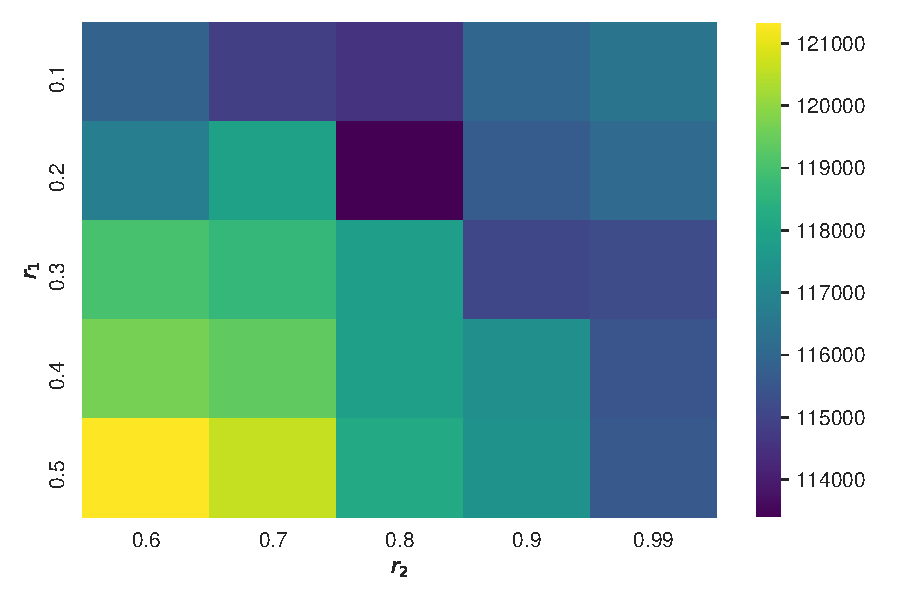
\includegraphics[width=\textwidth]{../img/heatmap_lop_IO_N-t59d11xx}
  \end{minipage}
  \begin{minipage}{0.49\linewidth}
    \centering
    \texttt{N-sgb75.02} (LOP)\\[-0.2ex]
 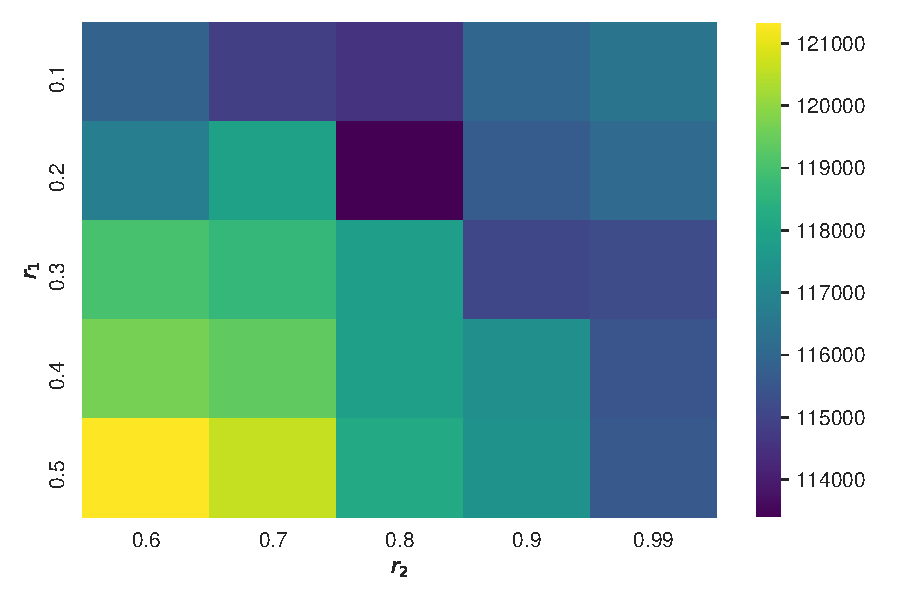
\includegraphics[width=\textwidth]{../img/heatmap_lop_SGB_N-sgb75_02}
\end{minipage}\\\vskip 1em
\begin{minipage}{0.49\linewidth}
  \centering
  \texttt{reC13} (PFSP)\\[-0.5ex]
  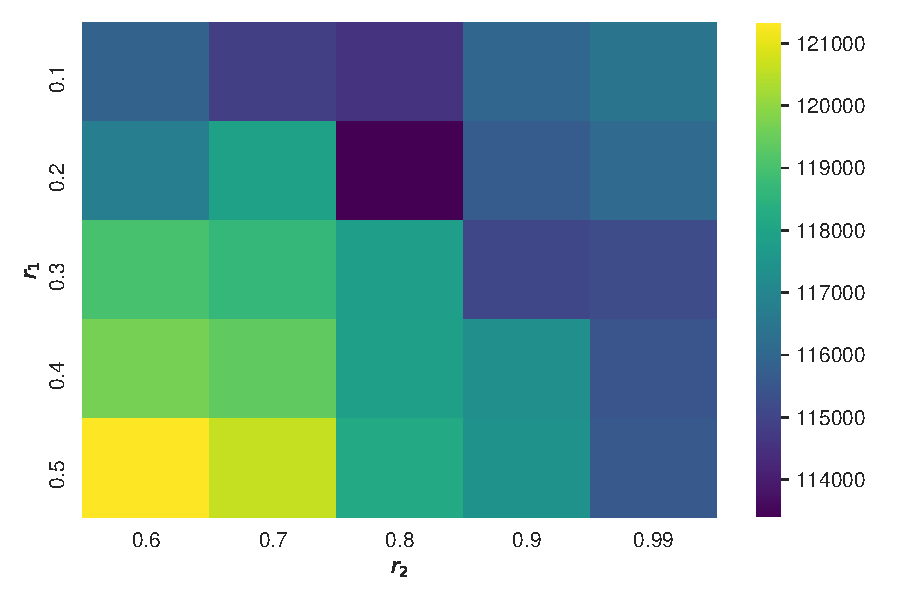
\includegraphics[width=\textwidth]{../img/heatmap_pfsp_rec13_txt}
\end{minipage}
\begin{minipage}{0.49\linewidth}
  \centering
  \texttt{reC19} (PFSP)\\[-0.5ex]
  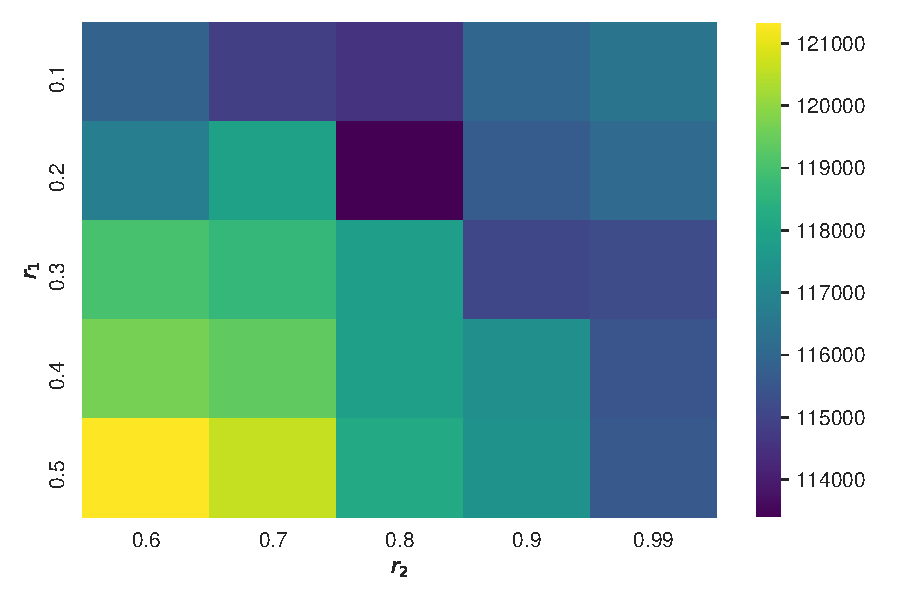
\includegraphics[width=\textwidth]{../img/heatmap_pfsp_rec19_txt}
\end{minipage}
% \begin{minipage}{0.49\linewidth}
%   \centering
%   \texttt{kra32} (QAP)\\[-0.5ex]
% 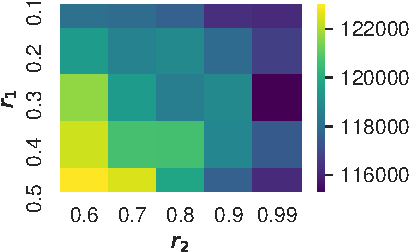
\includegraphics[width=\textwidth]{../img/heatmap_kra32_dat}
% \end{minipage}
\caption{Mean fitness (over 10 runs) of different configurations of $r_1$ and $r_2$ (darker is better).\label{fig:heatmaps}}
\end{figure}

The plot shows that UMM is indeed very sensitive to the values of $r_1$ and
$r_2$, yet, low values of $r_1$ and high values of $r_2$ almost always produce
the best results, independently of the problem.  In particular, we observe that
the pattern on the two top figures differs from the two bottom ones. While on
the top figures the fitness gets worse homogeneously from the top-right corner
to the bottom-left one, the pattern on the bottom figures is not as homogeneous, yet
still fitness gets worse with decreasing $r_2$.  We observe that this behavior
is related to the adequacy of UMM to the problem: the homogeneous behavior of
parameters $r_1$ and $r_2$ depends on the problem (not on the particular
instances) and the more homogeneous the behavior, the better performance of
UMM. We elaborate this argument in detail in the next section.

From this preliminary experiment, it is not obvious how the best settings are
related to problem features, such as permutation length ($n$). On the other
hand, given the sharp transitions in the plots, it is clear that further
fine-tuning may improve performance and uncover further patterns.

Over all the instances, we observe that the configuration $r_1 =0.1$, $r_2=0.9$
has good performance, i.e., its mean rank (over 10 runs) relative to all the
other configurations is less than 4 for all the instances.  Although automatic
parameter tuning may likely provide even more fine-tuned settings, our goal
here is to understand how UMM performs in comparison to an existing Bayesian
method (CEGO) and automatically tuning the parameters of CEGO is not
computationally feasible.  For consistency, in the following sections, we run
UMM with this parameter configuration.  Moreover, we recommend this
configuration as the current default of UMM.

%\subsection{Analysis of UMM and CEGO on synthetic LOP instances}
%
%To better understand the behavior of the algorithms, we record the fitness of
%the solution evaluated at each step of each run and we average those values
%over 10 runs with different random seeds on the same problem instance.  As an
%example, each line in Fig.~\ref{fig:lop_synth} shows the mean fitness of the
%solutions evaluated by either UMM or CEGO on one synthetic LOP instance. The
%shaded area shows one standard deviation around the mean. Ideally, each new
%evaluation will monotonically improve in fitness, since each solution evaluated
%helps to refine the model and leads to a better solution being evaluated in the
%next step.  However, it is possible that new solutions are worse
%than their predecessors. %Nevertheless, in this example, there is a clear
%% overall improvement as more evaluations are performed.
%The minimum values
%achieved in the plot up to a particular number of function evaluations gives an
%estimation of the mean fitness of the best-so-far solution up to that point in
%the run. The algorithms do not return the final solution shown but rather the
%best one (minimum fitness) of each run.
%
%
%%: LOP syntéticas, todas en una gráfica. 
%\begin{figure}[tb]
%  \centering%
%  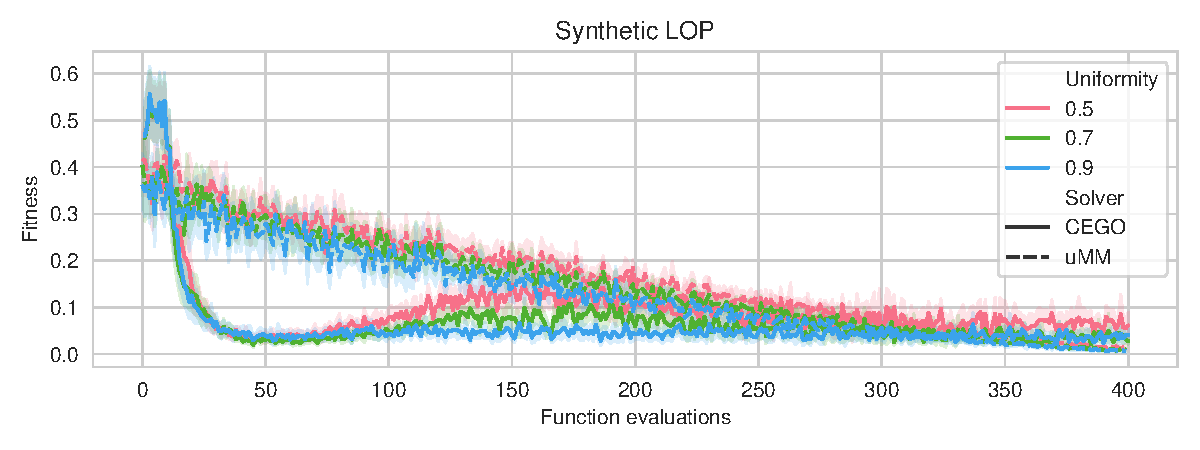
\includegraphics[width=\textwidth]{../img/synthetic_LOP_combined}
%  \caption{Mean fitness  (and standard deviation)  of each solution evaluated by each algorithm on LOP synthetic instances.\label{fig:lop_synth}}
%\end{figure}
%
%When we compare the behavior of CEGO and
%UMM on synthetic LOP instances (Fig.~\ref{fig:lop_synth}), we observe a clear
%pattern independently of the uniformity of the instances. In particular, we see
%a linear convergence to the optimal value for UMM.  This is due to the linear
%decrease in the parameter $\theta$ (line~\ref{line:theta} in
%Algorithm~\ref{alg:umm}), which imposes a linear variance decrease on the
%internal probability model of the UMM over the $\FEmax$ functions
%evaluations. Overall, the mean fitness returned by UMM at $\FEmax=400$ is better than the one returned by  CEGO, regardless the uniformity of the instances.
%
%
%
%%UMM converges much more slowly than CEGO, only reaching the
%%same fitness values around evaluation 250. 
%
%%Yet, UMM is able to keep the rate of
%%improvement and completely overtake CEGO around evaluation 350. As in the case
%%of CEGO, lower uniformity values lead to worse performance, although the
%%difference is much smaller for UMM than it was for CEGO.\MANUEL{If there is anything else we can say here, please go ahead and say it}
%
%On the other hand, % \EKHINE{cambio el orden}
%CEGO starts with 10 random initial solutions, % with are quite poor as
%% expected,
%followed by building and updating the Kriging model based on new
%evaluations, which leads to an impressive improvement in less than 50
%evaluations. However, progress is halted at this point and CEGO seems to
%have trouble finding better solutions. Around evaluation 200, the search
%becomes fully random. Lower uniformity values, e.g., 0.5, show worsening
%evaluations despite the increase in the number of solutions used to build the model. In
%summary, the Kriging model clearly helps CEGO to quickly identify good
%solutions in very few evaluations. However, CEGO is not able
%to further improve those solutions given more data. Given what we know about
%Kriging~\citep{EriPeaGar2019scalable}, it appears that the surrogate model cannot model the local step
%necessary to reach the optimal solution and switches to an exploration strategy
%that ends up being completely random.
%
%% This may due to the model not being able to produce accurate
%% predictions or the underlying optimizer not being able to find improved
%% solutions using the model.
%%\MANUEL{perhaps we should measure the
%%  prediction error and see if it grows or decreases. That would answer this
%%  question.}
%
%
%
%%: LOP reales: he puesto 3 de diferentes tamanos. Me ha parecido interesante que, a pesar de que CEGO parece que va mejor, esta diferencia se va reduciendo segun se aumenta el tamano del problema (que se puede ver en el nombre del problema y en el títutlo de la gráfica)
%\begin{figure}[!tb]
%  \centering%
%  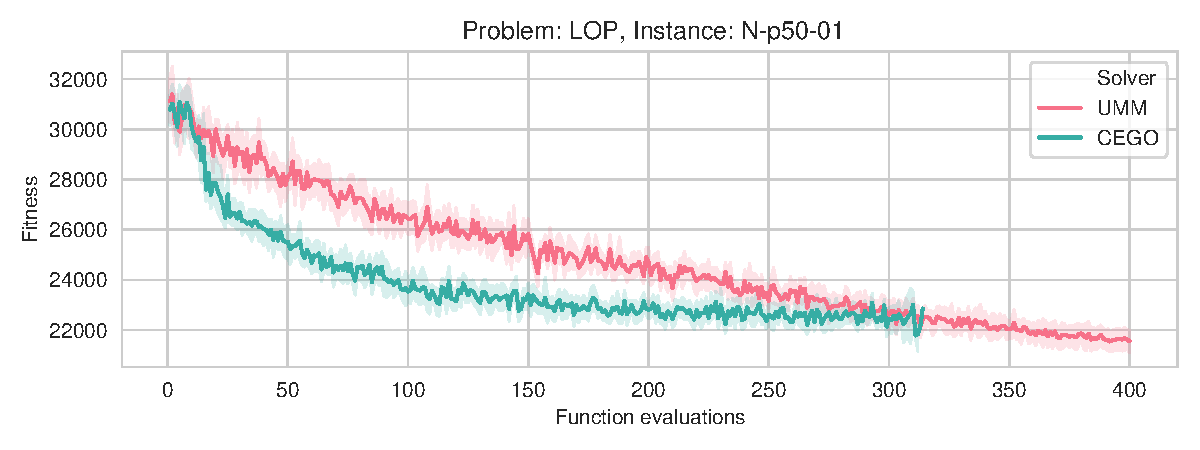
\includegraphics[width=\textwidth]{../img/fitness_real_lop_RandB_N-p50-01}\\
%  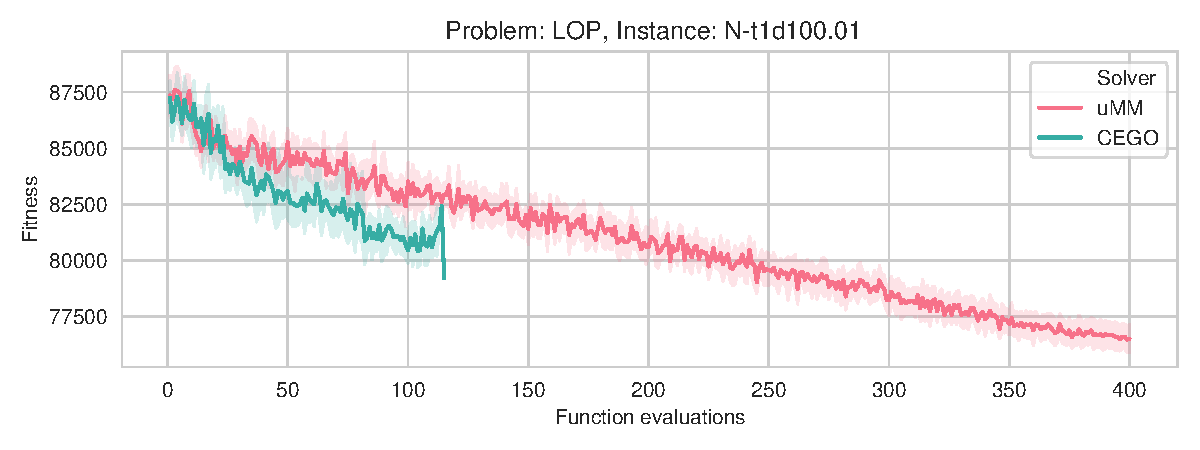
\includegraphics[width=\textwidth]{../img/fitness_real_lop_RandA1_N-t1d100_01}\\
%  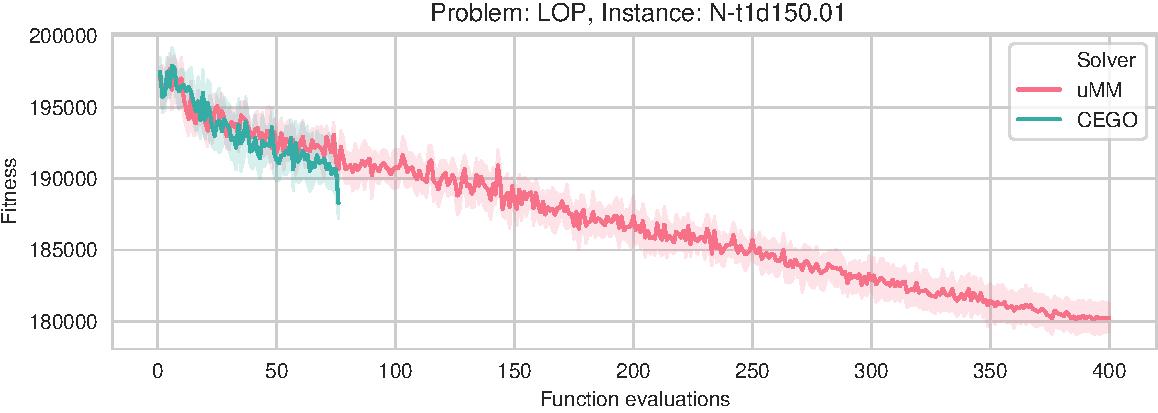
\includegraphics[width=\textwidth]{../img/fitness_real_lop_RandA1_N-t1d150_01}\\
%%  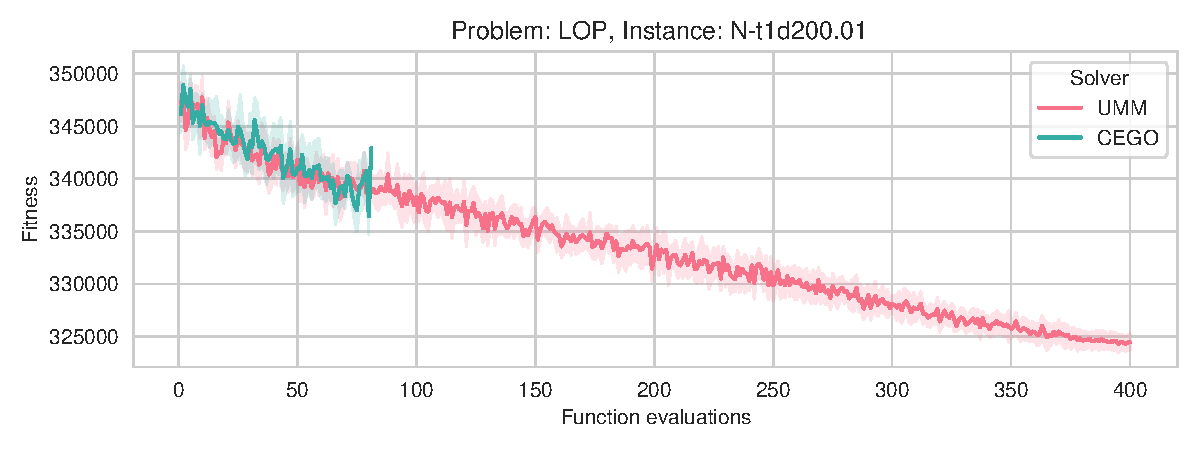
\includegraphics[width=\textwidth]{../img/fitness_real_lop_RandA1_N-t1d200_01}\\
%    \caption{Mean fitness  (and standard deviation)  of each solution evaluated by each algorithm on three instances from LOLIB.\label{fig:lolib}}
%  \end{figure}
%

%Results are quite different on the 
%The fast initial convergence of CEGO for synthetic LOP instances does not seem
%to translate to the
%instances available in LOLIB~\citep{}. We show in
%Fig.~\ref{fig:lolib} three examples with different permutation size, however,
%the results are consistent for other LOLIB instances (complete results
%available as supplementary material \supplement). Due to extremely long
%runtimes of CEGO and constraints in our computing system, we set a maximum
%wall-clock time of 3 days for each run of CEGO. On these instances, the
%behaviour of CEGO and UMM is much more similar (at least up to the termination
%point of CEGO). It appears that our synthetic LOP instances have a fitness
%landscape that is very amenable to CEGO's Kriging model, whereas the LOLIB
%instances do not present such landscape. Comparing CEGO and UMM results, the
%differences get smaller, in favour of UMM, with larger instance size. Our
%conjecture is that building an accurate Bayesian model and searching for good
%solutions on it becomes harder for larger fitness landscapes.
%\EKHINE{Parece que el paper va del CEGO en vez del UMM :p. Yo diría que tanto UMM como CEGO encuentran soluciones que mejoran según avanzan, pero con diferencias de comportamiento: (1) las los optimos de UMM son '3 veces mejor', y esto yo creo que es importante, aunque en gran parte se debe a que (2) UMM hace 400 ejecuciones en 3, 6 y 11 horas y CEGO entre 50 y 130 en 5 dias (3) cego empeora segun n aumenta (y n=200 tampoco es enorme)}
%\MANUEL{Eso es porque puedo interpretar los resultados de CEGO mejor que los de UMM. Si crees que hay alguna interpretación o conjetura sobre UMM que podemos mencionar aquí, sería bueno mencionarla.}
%\MANUEL{Prefiero dejar el comentario sobre las mejores soluciones encontradas y el tiempo requerido para cuando hable de la tabla, así se puede ver todo junto}



\subsection{Rankings and orderings}
In Section~\ref{sec:permutations} we highlighted the great difference of rankings and orderings, usually ommitted in the literature. In this lines, we show the consequences of misinterpreting permutations. We remind the reader that statistical models (Borda or the \ken distance) are defined for rankings while standard literature in optimization considers orderings. This is the reason while in the optimization field we will usually find the Swap distance instead of the \ken distance. However, both are usually claimed to be the same, which is false: they are the same in particular cases, for example when  one of the permutations is the identity or an inversion. 

As a summary of Algorithm~\ref{alg:umm}, we model rankings in our UMM model, generate a ranking $\sigma$, then invert this ranking to obtain an ordering in line~\ref{line:inversion} and evaluate the ordering $\sigma^{-1}$ in the objective function. This might seem an implementation detail but for the sake of consistency with the literature, we will expect objective functions to evaluate ordering. A natural question is what happens if we did not invert the ranking and evaluated a ranking with an optimization for orderings. For the anxious reader, we advance that the result is similar to the original version of CEGO. 


In CEGO, the objects modeled and evaluated are the same. They claim that they use the swap distance but they are using the \ken  distance, meaning that the object model is a ranking. \ekhine{}{esto es demasido rude?}
On the function evaluation the authors interpert their permutation as an ordering, as usual. 
However, there is no inversion between the objects sampled from the model and the objects evaluated. 
This means that both are rankings (or both are orderings). A natural question is what happens if we did invert the ranking. We have carried out all the experimentation with this modification of CEGO and we have denote this version CEGO\_inv. The original version of CEGO is denoted CEGO\_orig. 



%Figure~\ref{fig:rankorder} answers the above two questions. In a setting as the one in previous sections, we find 4 different lines, for the evaluation of UMM and CEGO with and without inversion. We see that in case of No inversion (dashed lines) both UMM and CEGO do not seem to converge (despite we can see some decrease along iterations). When there is an inversion between modelling and evaluation both algorithms behave better. In this case, since UMM is set for a a linear decrease in the the scale parameter for the $m$ iterations, we see the linear decrease in the function evaluations. In CEGO, we see an abrupt decrease at the beggining which seems stuck at iteration 200. 




\subsection{Analysis of UMM and CEGO on LOP and PFSP}
To  understand the behavior of the algorithms, we record the fitness of
the solution evaluated at each step of each run and we average those values
over 10 runs with different random seeds on the same problem instance.  As an
example, each line in Fig.~\ref{fig:results} shows the mean fitness of the
solutions evaluated by either UMM or CEGO on one instance. The
shaded area shows one standard deviation around the mean. Ideally, each new
evaluation will monotonically improve in fitness, since each solution evaluated
helps to refine the model and leads to a better solution being evaluated in the
next step.  However, it is possible that new solutions are worse
than their predecessors. %Nevertheless, in this example, there is a clear
% overall improvement as more evaluations are performed.
The minimum values
achieved in the plot up to a particular number of function evaluations gives an
estimation of the mean fitness of the best-so-far solution up to that point in
the run. The algorithms do not return the final solution shown but rather the
best one (minimum fitness) of each run. This result summarization is not the classical. However, due to the limited number of function evaluations, we can have a better picture of the behaviour of the algorithm at each step. As a consequence, results displayed here are not comparable with the original paper of CEGO: for this comparison we provide in Table~\ref{table:fitness} the summary of the best solutions found by each algorithm. 

Figure~\ref{fig:lolib} shows the results on the real-world instances taken from LOLIB. 
  %% MANUEL: Ya dimos la URL arriba, así que no la repetiría aquí
  % \footnote{\url{http://grafo.etsii.urjc.es/optsicom/lolib/}}
%The type of instances differs greatly from the synthetic LOP instances, and,
%thus, so does the landscape. However, UMM shows a very similar behavior: 
We can see that for UMM there 
is a (close to) linear decrease of the fitness of new solutions over each new
evaluation. This suggests that UMM is able to model the fitness
landscape. Regarding CEGO, \ekhine{we observe a similar behavior to UMM for the first
50-100 evaluations, however, in several instances CEGO reaches the time limit
of 144 hours, so no observations can be made for longer budgets. In smaller
instances (e.g., Figure~\ref{fig:lolib}, top), CEGO again appears to stagnate.}{ the objective function decrease slowly?}

% \ekhine{In the case of the PFSP, the progress of both algorithms resembles a random search, as illustrated by the results
%  obtained on \texttt{rec05} (Fig.~\ref{fig:rec05}), which is the smallest PFSP
% instance considered here. The lack of any apparent convergence suggests that
% the models (both Bayesian and probabilistic) are not learning anything about
% the fitness landscape. Results for larger PFSP corroborate these conclusions (\supplement).}{}
% \manuel{Although previous studies~\citep{ZaeStoBar2014:ppsn} concluded
% that other distance measures are more suited than Kendall's-$\tau$ distance for
% the PFSP, the reported fitness differences between various distance metrics are
% small.
% Hence, we conjecture that the same behavior will be observed with other distance metrics.}{}\MANUEL{On second thought, I'm not sure we should say this, because we really have no idea and we actually hope it is not true.}
  



\begin{figure*}[tb]
  \centering%
    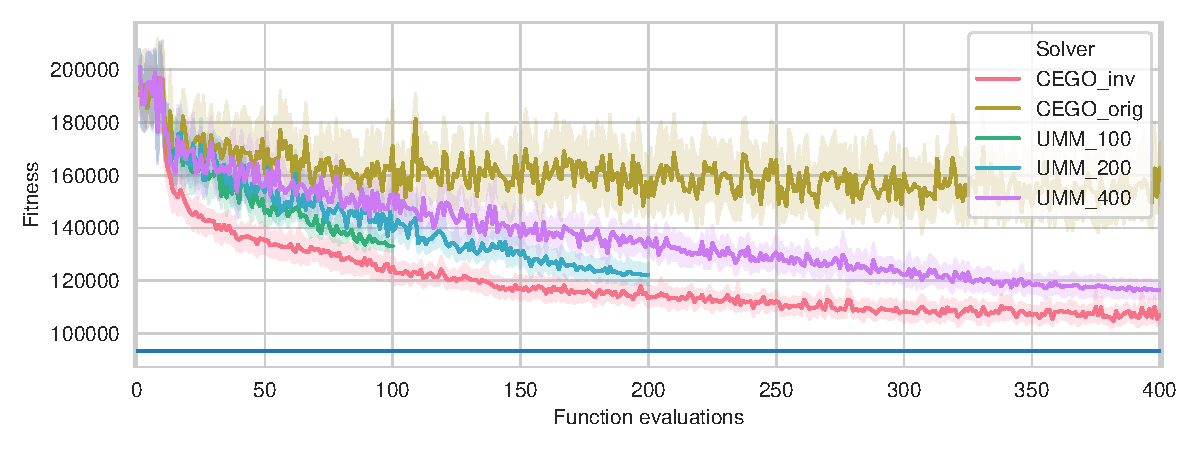
\includegraphics[width=0.49\textwidth]{../img/fitness_lop_IO_N-t59b11xx}
    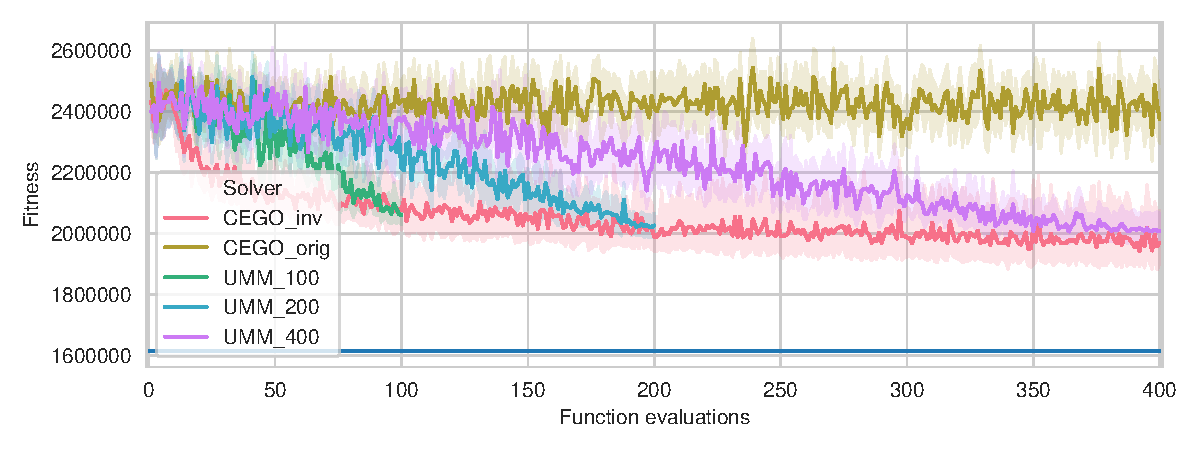
\includegraphics[width=0.49\textwidth]{../img/fitness_lop_SGB_N-sgb75_02}

    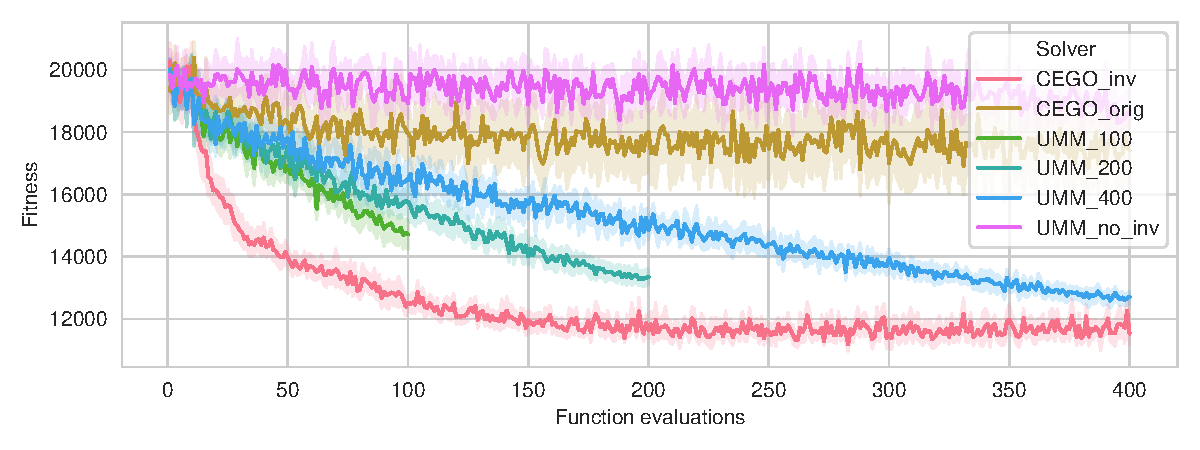
\includegraphics[width=0.49\textwidth]{../img/fitness_lop_RandB_N-p40-01}
    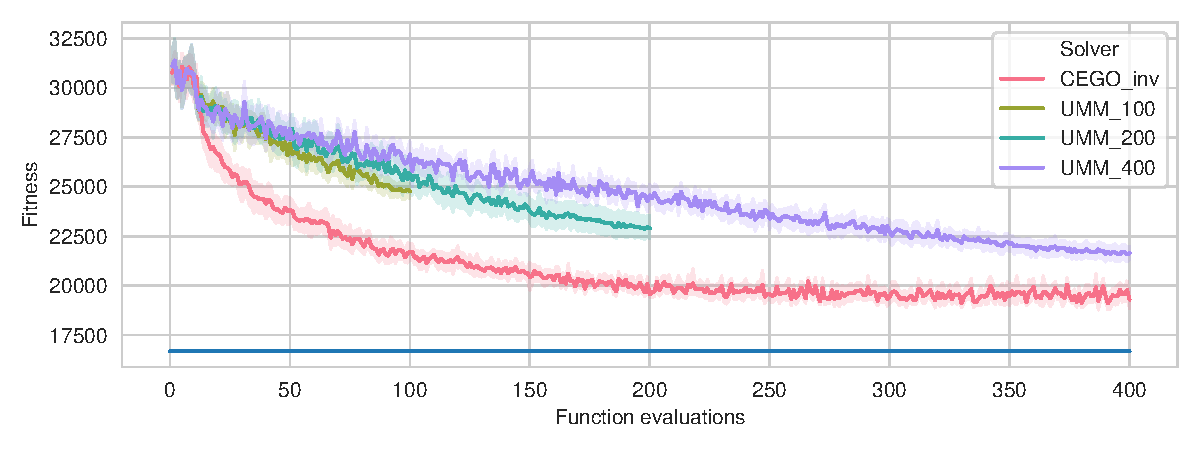
\includegraphics[width=0.49\textwidth]{../img/fitness_lop_RandB_N-p50-01}

    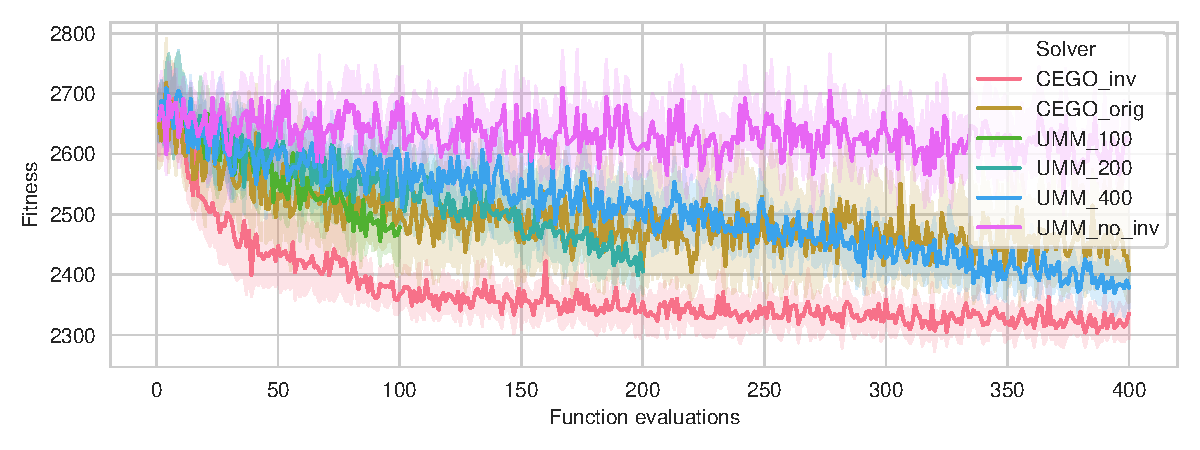
\includegraphics[width=0.49\textwidth]{../img/fitness_pfsp_rec19_txt}
    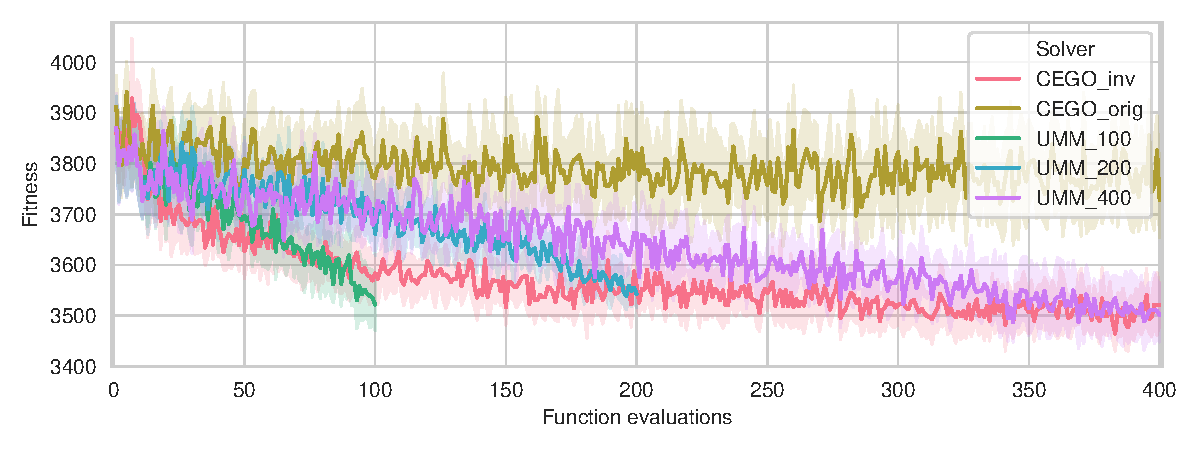
\includegraphics[width=0.49\textwidth]{../img/fitness_pfsp_rec31_txt}
\label{fig:results}
  \caption{Mean fitness  (and standard deviation)  of each solution evaluated by each algorithm on the PFSP instance \texttt{rec05}.\label{fig:rec05}}
\end{figure*}


% The situation is very similar for the QAP, where both algorithms show the same
% behaviour as in the PFSP for all instances tested, except for
% \texttt{kra} instances. As shown in Fig~\ref{fig:kra32}, for \texttt{kra32} both
% algorithms are able to improve over the number of evaluations, although not
% with ease. As in the synthetic LOP instances, we again observe that CEGO does
% improve faster than UMM initially, yet CEGO appears to get stuck around
% evaluation 250, and UMM overtakes it around evaluation 300. We believe the
% reason is the same as before, that is, the CEGO model is not able to adequately
% reflect the ruggedness of the actual landscape and, hence, the best solutions
% found by the GA searching the model are not improved solutions for the actual
% problem. Interestingly, there are well-known differences between
% \texttt{kra30a}, \texttt{kra30b}, \texttt{kra32}, on one hand, and \texttt{nug12}, \texttt{nug30} and
% \texttt{tho32}, on the other~\citep{AnsBriGou2002qap}. However, we cannot at
% this moment point out the root cause of this different behavior.

% \begin{figure}[tp]
%   \centering%
%   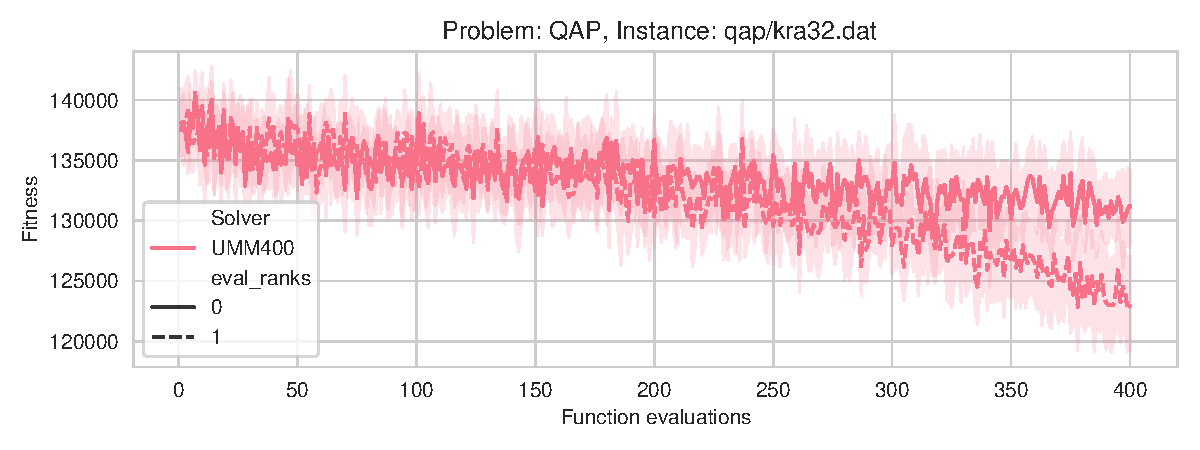
\includegraphics[width=\textwidth]{../img/fitness_real_qap_kra32_dat}
%   \caption{Mean fitness  (and standard deviation)  of each solution evaluated by each algorithm on the QAP instance \texttt{kra32}.\label{fig:kra32}}
%   \vspace*{-1em}
% \end{figure}

Table~\ref{tab:results} shows results over all instances evaluated (excluding
the synthetic LOP instances). In particular, we show the mean fitness (and
standard deviation) of the best solution found at the end of each run. We also report the mean runtime in hours and, since CEGO sometimes reached the limit of 144 hours, also the number of fitness evaluations reached by CEGO.

In the LOP, differences are mostly in favour of UMM, due to the time limit of
144 hours, which resulted in CEGO typically achieving less than 200
evaluations. In contrast, UMM was always able to reach 400 evaluations in less
than 12.5 hours. If UMM was allowed to reach the 144 hours limit, the differences
would be even stronger.
%
In the PFSP, the differences are minor and/or not statistically
significant, with the qualification that both algorithms appear to be
performing a random search.

The overall conclusion from Table~\ref{tab:results} is that there is not a
significant difference in performance between UMM and CEGO. For the larger LOP
instances, CEGO reaches the time limit of 144 hours before consuming the budget
of 400 evaluations and thus, obtains quite poor solutions compared to UMM,
which is at least an order of magnitude faster.



% Please add the following required packages to your document preamble:
% \usepackage{multirow}
\begin{table*}[]
\begin{tabular}{rrrrrrrrr}
\multicolumn{1}{c}{\textbf{}} & \multicolumn{1}{c}{\textbf{}} & \multicolumn{4}{c}{\textbf{Mean fitness (sd)}}                       & \multicolumn{1}{c}{\multirow{2}{*}{\textbf{\begin{tabular}[c]{@{}c@{}}95\% CI of the \\ mean difference\end{tabular}}}} & \multicolumn{2}{c}{\textbf{Runtime}} \\ \cline{3-6} \cline{8-9} 
\textbf{Problem}              & \textbf{Instance}             & \multicolumn{2}{r}{\textbf{CEGO}} & \multicolumn{2}{r}{\textbf{UMM}} & \multicolumn{1}{c}{}                                                                                                    & \textbf{CEGO}     & \textbf{UMM}     \\ \hline
LOP                           & N-p40-01                      & 10496.6          & (116.8)        & 12369.1         & (389.9)        & {[}-2157.1, -1587.9{]}                                                                                                  & 19.9              & 0.3              \\
LOP                           & N-p40-02                      & 11714.7          & (84.7)         & 13160.5         & (454.8)        & {[}-1773.5, -1118.1{]}                                                                                                  & 20.1              & 0.3              \\
LOP                           & N-t59b11xx                    & 102408.0         & (3800.2)       & 114075.5        & (5389.2)       & {[}-16084.2, -7250.8{]}                                                                                                 & 21.1              & 0.4              \\
LOP                           & N-t59d11xx                    & 12692.2          & (1097.9)       & 16662.9         & (2155.3)       & {[}-5618.5, -2322.9{]}                                                                                                  & 21.2              & 0.4              \\
LOP                           & N-p50-02                      & 19090.5          & (285.4)        & 21746.6         & (645.4)        & {[}-3140.6, -2171.6{]}                                                                                                  & 22.9              & 0.5              \\
LOP                           & N-p50-01                      & 18197.7          & (225.6)        & 21161.8         & (657.4)        & {[}-3447.4, -2480.8{]}                                                                                                  & 23.2              & 0.5              \\
LOP                           & N-sgb75.01                    & 1893533.2        & (28594.6)      & 1992059.9       & (40235.7)      & {[}-131577.1, -65476.3{]}                                                                                               & 33.2              & 1.0              \\
LOP                           & N-sgb75.02                    & 1895801.8        & (82847.9)      & 1967132.3       & (49228.1)      & {[}-136421.2, -6239.8{]}                                                                                                & 33.3              & 1.1              \\
PFSP                          & rec05                         & 1276.2           & (15.1)         & 1276.3          & (8.4)          & {[}-11.8, 11.6{]}                                                                                                       & 18.3              & 0.1              \\
PFSP                          & rec13                         & 1992.9           & (27.6)         & 2057.8          & (22.8)         & {[}-88.8, -41.0{]}                                                                                                      & 18.5              & 0.1              \\
PFSP                          & rec19                         & 2264.5           & (45.0)         & 2304.8          & (37.7)         & {[}-79.4, -1.2{]}                                                                                                       & 18.2              & 0.2              \\
PFSP                          & rec31                         & 3415.5           & (62.1)         & 3419.3          & (37.0)         & {[}-52.6, 45.0{]}                                                                                                       & 23.1              & 0.5             
\end{tabular}
\end{table*}



\begin{table*}[tb]%time
\begin{tabular}{llrrrrr}
\toprule
Problem &    Instance &  CEGO\_inv &  CEGO\_orig &  UMM\_400 &  UMM\_200 &  UMM\_100 \\
\midrule
    LOP &  N-t59b11xx &   1265.98 &    1240.36 &    22.24 &     5.78 &     1.37 \\
    LOP &  N-t59d11xx &   1269.93 &    1252.89 &    21.84 &     5.62 &     1.37 \\
    LOP &    N-p40-01 &   1195.90 &    1170.81 &    18.13 &     4.61 &     1.14 \\
    LOP &    N-p40-02 &   1207.24 &    1183.09 &    18.11 &     4.76 &     1.15 \\
    LOP &    N-p50-01 &   1391.55 &        NaN &    27.36 &      NaN &      NaN \\
    LOP &    N-p50-02 &   1372.71 &        NaN &    28.36 &      NaN &      NaN \\
    LOP &  N-sgb75.01 &   1994.22 &    2004.70 &    62.75 &    15.77 &     3.97 \\
    LOP &  N-sgb75.02 &   1995.09 &    1975.41 &    64.58 &    15.90 &     4.03 \\
   PFSP &       rec05 &   1099.63 &     917.81 &     4.54 &     1.14 &     0.30 \\
   PFSP &       rec13 &   1109.51 &    1043.08 &     4.55 &     1.07 &     0.31 \\
   PFSP &       rec19 &   1090.06 &    1087.38 &    10.51 &     2.59 &     0.63 \\
   PFSP &       rec31 &   1387.09 &    1367.26 &    27.84 &     6.90 &     1.79 \\
\bottomrule
\end{tabular}
\end{table*}


\begin{table*}[tb]%fitness
\begin{tabular}{llrrrrr}
\toprule
Problem &    Instance &   CEGO\_inv &   CEGO\_orig &   UMM\_400 &   UMM\_200 &   UMM\_100 \\
\midrule
    LOP &  N-t59b11xx &          102408.0 &           126204.0 &         114075.5 &         115941.5 &         128195.5 \\
    LOP &  N-t59d11xx &           12692.2 &            30199.8 &          16662.9 &          22117.4 &          28050.4 \\
    LOP &    N-p40-01 &           10496.6 &            15027.7 &          12369.1 &          13043.7 &          14459.3 \\
    LOP &    N-p40-02 &           11714.7 &            15150.2 &          13160.5 &          13923.2 &          15027.7 \\
    LOP &    N-p50-01 &           18197.7 &                NaN &          21161.8 &              NaN &              NaN \\
    LOP &    N-p50-02 &           19090.5 &                NaN &          21746.6 &              NaN &              NaN \\
    LOP &  N-sgb75.01 &         1893533.2 &          2095899.6 &        1992059.9 &        2011271.7 &        2074111.6 \\
    LOP &  N-sgb75.02 &         1895801.8 &          2069286.9 &        1967132.3 &        2011004.2 &        2045556.5 \\
   PFSP &       rec05 &            1276.2 &             1318.7 &           1276.3 &           1283.1 &           1300.4 \\
   PFSP &       rec13 &            1992.9 &             2096.0 &           2057.8 &           2113.6 &           2134.9 \\
   PFSP &       rec19 &            2264.5 &             2328.4 &           2304.8 &           2346.5 &           2392.4 \\
   PFSP &       rec31 &            3415.5 &             3512.3 &           3419.3 &           3438.9 &           3511.9 \\
\bottomrule
\end{tabular}
\end{table*}



\section{Conclusions}\label{sec:conclusions}

In this paper, we have introduced UMM, a population-based probabilistic
algorithm based on an unbalanced Mallows model. The algorithm is designed for
black-box combinatorial problems on permutation landscapes and when the budget
of fitness evaluations is severely limited (here, up to $400$ evaluations).
Our experiments presented here show that UMM is able to match the results of
CEGO, a state-of-the-art Bayesian optimizer for expensive black-box
optimization if the computation time of the optimizers is not a concern.

In addition, UMM is specially well-suited for budget-limited scenarios that are
still time-sensitive, e.g., when the overhead incurred by the optimizer should
be no more than a few minutes added to each fitness evaluation. By comparison,
CEGO may require up to one hour per fitness evaluation, with the time
increasing non-linearly with permutation size and larger budgets.  Hence, UMM
is a computationally feasible alternative for relatively large problem sizes.


%\MANUEL{UMM is able to model the LOP landscape
%  at least as well as CEGO as shown by the plots where UMM shows a linear
%  decrease in fitness.}  
%  \EKHINE{me parece mas de CEGO q UMM y parece q UMM
%  solo tiene de ventaja ir rápido. Primero destacaría lo bueno de UMM. Creo q
%  es importante destaacar q UMM va MEJOR o IGUAL en TODOS los experimentos y
%  luego que addemás es más rápido} 
%  \MANUEL{Pero UMM es peor en rec13 y nug12, y
%  en LOP es mejor porque CEGO no llega a 400, es decir, porque UMM es más
%  rápido. No podemos saber qué pasaría si CEGO llegara a 400. Podríamos medir
%  lo que pasa en el momento en que matamos a CEGO y dar también ese valor
%  entonces la diferencia en velocidad no importaría. } 
% The time required to train the surrogate-model of \ekhine{esta establecida la complexity de CEGO???}{UMM increases linearly with the permutation length $n$, while in }
% CEGO  it sharply
% increases with $n$, requiring 
% sometimes more than hour per fitness evaluation as shown in the experimental section. 
% Hence, UMM is a computationally
% feasible alternative for relatively large problem sizes.

Although we were inspired by previous work on ACO for expensive black-box
combinatorial problems~\citep{PerLopStu2015si}, UMM is, to the best of our
knowledge, the first EDA specifically designed for such problems that is able
to match (and sometimes even improve) the results of a Bayesian
optimizer. Moreover, it is overwhelmingly faster than the alternatives for
large problem sizes.  The results presented here show that, despite the
intrinsic difficulty of the expensive black-box combinatorial scenario, there
are still significant advances yet to be made. Thus, we hope that this paper
will motivate further research. % on such problems.
%\MANUEL{I'm thinking about finishing here and commenting out the following paragraph}

An interesting result is that the behavior of UMM (and the same for CEGO) on
the PFSP (and some QAP instances) is close to random. %The same behavior is
%observed for CEGO, which seems to have been never reported until now.
This result may be due to the distance
metric used, but further analysis is needed to corroborate this
conjecture. Here, we have focused on Kendall's-$\tau$ distance, however, we are certain it is
possible to extend UMM to other distance metrics, which will allow us to
dynamically select among various distance metrics for an unknown black-box
% \ekhine{}{estoy totalmente en contra de esto :) }
permutation landscape~\citep{ZaeStoBar2014:ppsn}. Also, as shown by our
experiments, the behavior of the parameters ($r_1$ and $r_2$) of UMM is not
always obvious, thus a more detailed analysis would be needed to provide either
generally good static values or an online adaptation approach. Finally, we have
used here three very different combinatorial problems (LOP, PFSP and QAP) as
black-box benchmarks. However, an even more diverse range of problems would be
needed to understand the behavior of UMM on real-world black-box combinatorial
landscapes.


% Bayesian optimization methods using a global GP model, such as CEGO, are known
% to have trouble optimizing locally \citep{EriPeaGar2019scalable}. Our
% intuition is that this problem becomes worse in rugged combinatorial
% landscapes, where small steps may produce drastic changes.

% Open questions:
% \begin{itemize}
% \item How difficult is to extend UMM to other distance metrics?
% \item Can we plot the posterior probability of the optimal solution?
% \end{itemize}

\subsubsection{Reproducibility} Source code, datasets and scripts necessary to reproduce the results are available at \supplement.
%  \vspace*{-1em}
%\begin{acks}
%% MANUEL: Blind, so no acknowledgments yet.
%\paragraph*{Acknowledgements.} Blind
% M.\@ L\'opez-Ib\'a\~nez is a ``Beatriz Galindo'' Senior Distinguished Researcher (BEAGAL 18/00053) funded by the Ministry of Science and Innovation of the Spanish Government.
%
%\manuel{}{: We should also thank the COST ACTION: Ask Carlos?} \ekhine{}{Sure!, esto no habra q ponerlo aun por ser blind, no?}
%Thanks to: Hao Wang (Leiden University) for pointing us to the arguments of
%\citep{EriPeaGar2019scalable}; Thomas Stützle (Université libre de Bruxelles) for suggesting works
%about differences between QAPLIB instances; and Ahmed Boujaada for the experimental support. 
  % supported by the \grantsponsor{GS501100001809}{National Natural
  %   Science Foundation of
  %   China}{http://dx.doi.org/10.13039/501100001809} under Grant
  % No.:~\grantnum{GS501100001809}{61273304}
  % and~\grantnum[http://www.nnsf.cn/youngscientists]{GS501100001809}{Young
  %   Scientists' Support Program}.
%\end{acks}

%\renewcommand{\doi}[1]{doi:\hspace{.16667em plus .08333em}\discretionary{}{}{}\href{https://doi.org/#1}{\urlstyle{rm}\nolinkurl{#1}}}

\bibliographystyle{ACM-Reference-Format-abbrv}
\bibliography{optbib/abbrev,optbib/authors,optbib/abbrevshort,optbib/journals,optbib/biblio,optbib/crossref}%,./mendeley}

\end{document}

%%% Local Variables:
%%% mode: latex
%%% TeX-master: t
%%% End:
